\section{Advanced Topics in Deep Learning for Computer Vision}

\subsection{Recall on CNNs}

In representation learning we try to find good ways of representing data, often by learning a useful transformation of the raw data.
Deep learning is a subset of representation learning.

\subsubsection{Gradient descent}
Neural networks are usually trained using iterative, gradient-based optimizers that drive the cost function to a very low value.
The convergence point of gradient descent depends on the initial values of the parameters.
For feedforward neural networks it's important to initialize all weights to small random values and to initialize biases to zero or to small positive values.
To apply gradient based learning we must choose a cost function and how to represent the output of the model.
The derivative $f'(x)$ gives the slope of $f(x)$ at the point $x$.
The derivative is useful for minimizing a function because it tells us how to change $x$ in order to make a small improvement in $y$.
A point that obtains the absolute lowest value of $f(x)$ is a global minimum.

To reach the minimum we use the formula $w' = w - \alpha \frac{\partial J(w,b)}{\partial w} \,\, b' = b - \alpha \frac{\partial J(w,b)}{\partial b}$, where $\alpha$ is the learning rate, which controls how big are the steps that we take during the gradient descent.
If the slope is positive, we subtract the quantity in order to reach the minimum, or else we do the opposite thing.

As the training set size grows to billions of examples, the time to take a single gradient step becomes prohibitively long.
Stochastic/Minibatch gradient descent are extensions of the gradient descent algorithm. We can sample a minibatch of examples drawn uniformly from the training set (1 for stochastic).
It's like training every time on a different (smaller) training set.

\paragraph{Optimizers: momentum}
Momentum was designed to accelerate learning, especially in the face of high curvature, small but consistent gradients, or noisy gradients.
The size of the step depends on how large and how aligned a sequence of gradients are.
The step size is largest when many successive gradients point in the same direction.
Momentum smooths the step of the gradient descent in its path to the minimum.
We compute: $W^{[l+1]} = W^{[l]} - \alpha v_{W^{[l + 1]}}$, where $v_{W^{[l + 1]}} = \beta v_{W^{[l]}} + (1-\beta) \frac{\partial J(...)}{\partial W^{[l]}}$.
Root Mean Square Propagation (RMSprop) uses an exponentially decaying average to discard history from the extreme past so that it doesn't impede the convergence.

\paragraph{Optimizers: Adam}
The name derives from "adaptive moments", and it can be seen as the combination of RMSprop and momentum.
It's fairly robust to the choice of hyperparameters, though the learning rate sometimes needs to be changed from the suggested default.
There is a first order and a seond order Adam.
The first order Adam uses the gradient and its moving averages (first moments) to update the parameters.
The second order Adam incorporates information about the curvature of the loss surface, using approximations of the Hessian or second order derivatives, which leads to more informed and potentially more efficient updates but requires more computational resources.

\subsubsection{Convolutions and filters}
An image is characterized by height, width and number of channels.

\begin{figure}[htbp]
  \centering
  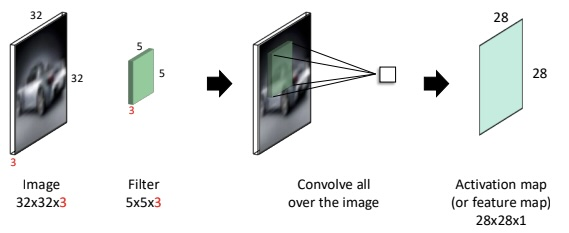
\includegraphics[width=0.8\linewidth]{./img/convolution_filter.jpg}
  \caption{A convolutional filter has the \textbf{same depth} of the input volume, so the output dimension is 1.}
  % \label{fig:forward_mapping}
\end{figure}

We can also train more than one filer, where each filter outputs a feature map.
By stacking activation maps we get a new volume.

Since convolutions shrink the images we can use padding to preserve the edges.
We have always considered a stride of 1 (moving the convolutional filter by one pixel), but we can also use different stride sizes to shrink the image.

\begin{figure}[htbp]
  \centering
  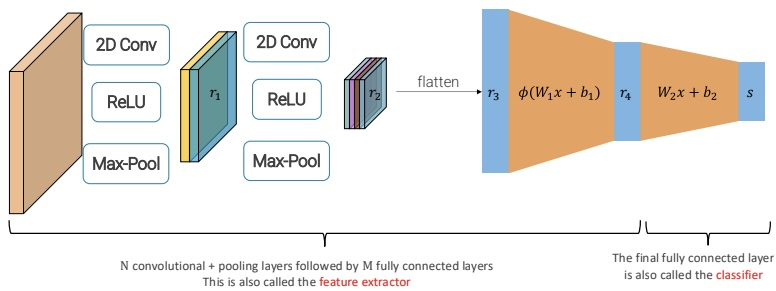
\includegraphics[width=0.8\linewidth]{./img/deep_cnn.jpg}
  \caption{By stacking together convolutional filters, pooling layers and fully connected layers we can design a Deep CNN.}
\end{figure}

\paragraph{Pooling}
A pooling layer is used to reduce the size of the representation in order to speedup computation.
Pooling comes usually after each conv layer or after a block (or set) of conv layers.
It's applied to each activation map independently.

\begin{figure}[htbp]
  \centering
  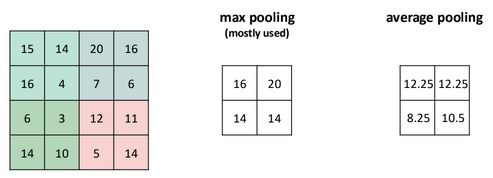
\includegraphics[width=0.8\linewidth]{./img/pooling.jpg}
  \caption{Example: pooling of dimension 2 and stride 2.}
\end{figure}

\paragraph{Receptive fields}
The input pixels affecting a hidden unit are called its receptive field.
We can encode the information in all the pixels to a single point.
We go from spatial to semantic information (we transform spatial information to semantic information).

\paragraph{Convolution parameters and flops}

\begin{figure}[htbp]
  \centering
  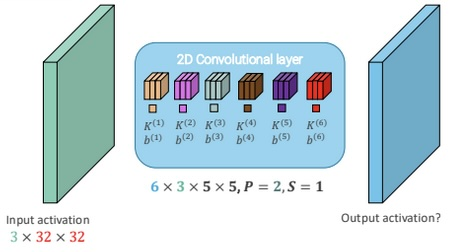
\includegraphics[width=0.8\linewidth]{./img/convolutions_flops.jpg}
  \caption{}
  \label{fig:convolutions_flops}
\end{figure}

As we can see in \ref{fig:convolutions_flops}, the number of learnable parametes for the convolutional layer is $6 \times (3 \times 5 \times 5 + 1) = 6 \times 76 = 456$ (6 convolutional blocks, 3 channels per convolutional block, $5 \times 5$ convolution, ).
The size of the output is $H_\text{{out}} = W_\text{{out}} = 32 - 5 + 2 * 2 + 1 = 32$.
Hence, there are $6 \times 32 \times 32 = 6144$ values in the output activation ($\approxeq 24$KB).

Since each of them is obtained as the dot product between the weights and the input, which requires to perform $n$ multiplications and $n$ summations for inputs of size $n$, i.e. $2n$ flops.

\subsubsection{Batch Normalization (BatchNorm)}
BatchNorm is a technique designed to stabilize and accelerate the training of deep neural networks by addressing internal covariate shift: the change in the distribution of layer activations caused by updates to preceding layers during training.
By normalizing activations at each layer, BatchNorm ensures that gradients are propagated more effectively, enabling coordinated updates across deep networks.

Let $Z^{[l]}$ be a minibatch of activations of the $l$-th layer to be normalized.
To normalize $Z^{[l]}$, we replace it with: $Z^{[l]}_{norm} = \frac{Z^[l] - \mu}{\sigma}$, where $\mu$ is a vector containing the mean of each unit and $\sigma$ is a vector containing the mean of each unit and $\sigma$ is a vector containing the standard deviation of each unit.
$\mu$ and $\sigma$ are running averages of the values seen during training.
BatchNorm helps with speeding up the training, and has a slight regularization effect (but we don't use it for this reason).

We use LayerNorm for fully connected layers because it normalizes per sample, making it batch-size independent.
We use InstanceNorm for convolutional layers because it normalizes per sample and per channel.

\subsubsection{Dropout regularization}
Dropout randomly deactivates a fraction of neurons during training, effectively training an ensemble of smaller sub-networks.
For each layer, you set a dropout probability, determining the chance a neuron is ignored in a forward pass.
This helps to prevent overfitting because we don't associate a certain pattern to a certain output of the network.

\begin{figure}[htbp]
  \centering
  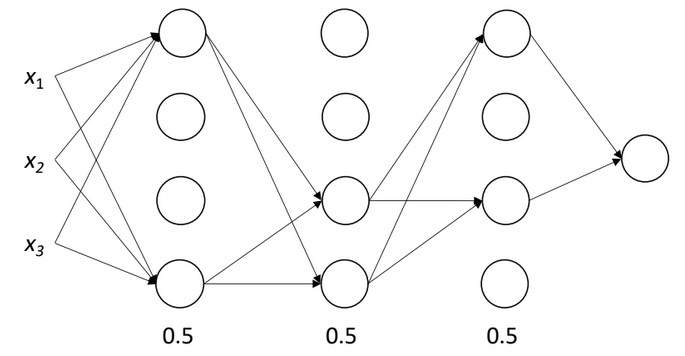
\includegraphics[width=0.8\linewidth]{./img/dropout.jpg}
  \caption{Each layer has a $50 \%$ dropout probability}
  \label{fig:dropout}
\end{figure}

Dropout and normalization are used only at training time.
When we test the network we switch off dropout and regularization.

Another powerful regularization technique is just having more data.

\subsubsection{Data augmentation}
We can create more data by modifying the images we already have.
We must only make transformations which keep the labels valid.
We can, for example, sample random crops/scales of the data or do color augmentation.

Cutout is the process where we remove a random square region of the input image.
This forces the network to use a more diverse set of features, helping generalization.
It's gray because we subtract the mean from this pictures, and so the number in the cutout becomes 0.

\subsection{CNNs}

\subsubsection{AlexNet \& ZFnet}
In 2012 Alex Krizhevsky proposed AlexNet, which had almost a $9\%$ of improvement on SOTA.

\begin{figure}[htbp]
  \centering
  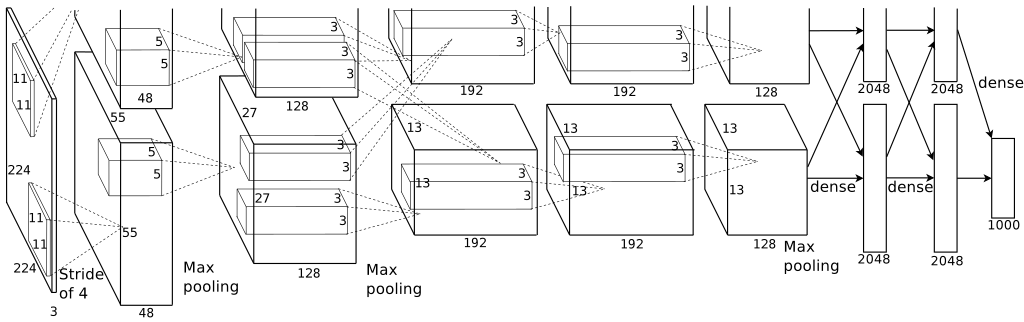
\includegraphics[width=0.8\linewidth]{./img/alexnet.png}
  \caption{AlexNet architecture}
  \label{fig:alexnet}
\end{figure}

In the image \ref{fig:alexnet}, we see only one half of the network, since the architecture is replicated identically 2 times to be used on a 2 GPU setup.
The network is composed by a \textbf{stem layer} at the beginning, which is a convolution layer that performs a fast reduction in the spatial size of the activations, mainly to reduce memory and computational cost.
The first layer has two $11 \times 11$ kernels, which extracts corners/edges/blobs.

To counteract these problems ZFnet used $7\times 7$ convolutions with stride 2 in the first layer and $5\times 5$ convolutions with stride 2 also in the second convolutional layer.

\subsubsection{VGG}
To avoid the vanishing gradient problem VGG used $3 \times 3$ convolutions only, and didn't use the stem layer.
The network was shallower, and used only convolutions and pooling.
At the end it used the same flattening and classification head.

Pre initialization with weights from shallower architectures was crucial to let the training progress, since batch normalization wasn't yet invented.

\begin{figure}[htbp]
  \centering
  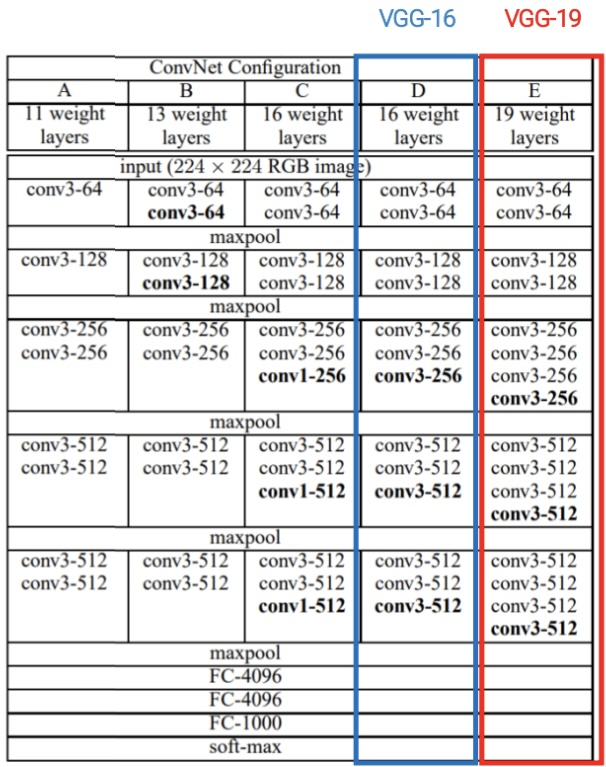
\includegraphics[width=0.35\linewidth]{./img/vgg.jpg}
  \caption{VGG architecture}
  % \label{fig:alexnet}
\end{figure}

VGG introduces the idea of designing a network as repetition of stages, i.e. a fixed combination of layers that process activations at the same spatial resolution.
In VGG we have 3 types of blocks:
\begin{itemize}
  \item \verb|conv-conv-pool|.
  \item \verb|conv-conv-conv-pool|.
  \item \verb|conv-conv-conv-conv-pool| (we can get a more complex convolution by combining $3\times 3$ convolutions).
\end{itemize}

One stage has the same receptive field of larger convolutions but requires less parameters and computation, and introduces more non-linearities.

The disadvantage is that the memory for activation doubles.

\begin{table}[htbp]
\begin{tabular}{|l|l|l|l|l|}
\hline
convolutional layer                                    & params       & flops                 & ReLUs & number of activations                \\ \hline
$C \times C \times 5 \times 5, \,S=1,\, P=2$           & $25C^2 + C$  & $50C^2 W_{in} H_{in}$ & 1     & $C\times W_{in} \times H_{in}$ \\ \hline
2 stacked $C \times C \times 3 \times 3, \,S=1,\, P=1$ & $18C^2 + 2C$ & $10C^2 W_{in} H_{in}$ & 2     & $2\times C \times W_{in} \times H_{in}$ \\ \hline
\end{tabular}
\end{table}

VGG-16 is composed by 138M parameters ($2.3x$ AlexNet), mostly in fully connected layers.
The computational cost is $\approx 4$ Tflops, mainly due to convolutions, and the network uses about $\approx 16.5$ GB of memory.

\subsubsection{Inception v1 (GoogLeNet)}
The main hallmark of this architecture is the improved utilization of the computing resources inside the network.
This was achieved by a carefully crafted design that allows for increasing the depth and width of the network while keeping the computational budget constant.

\begin{figure}[htbp]
  \centering
  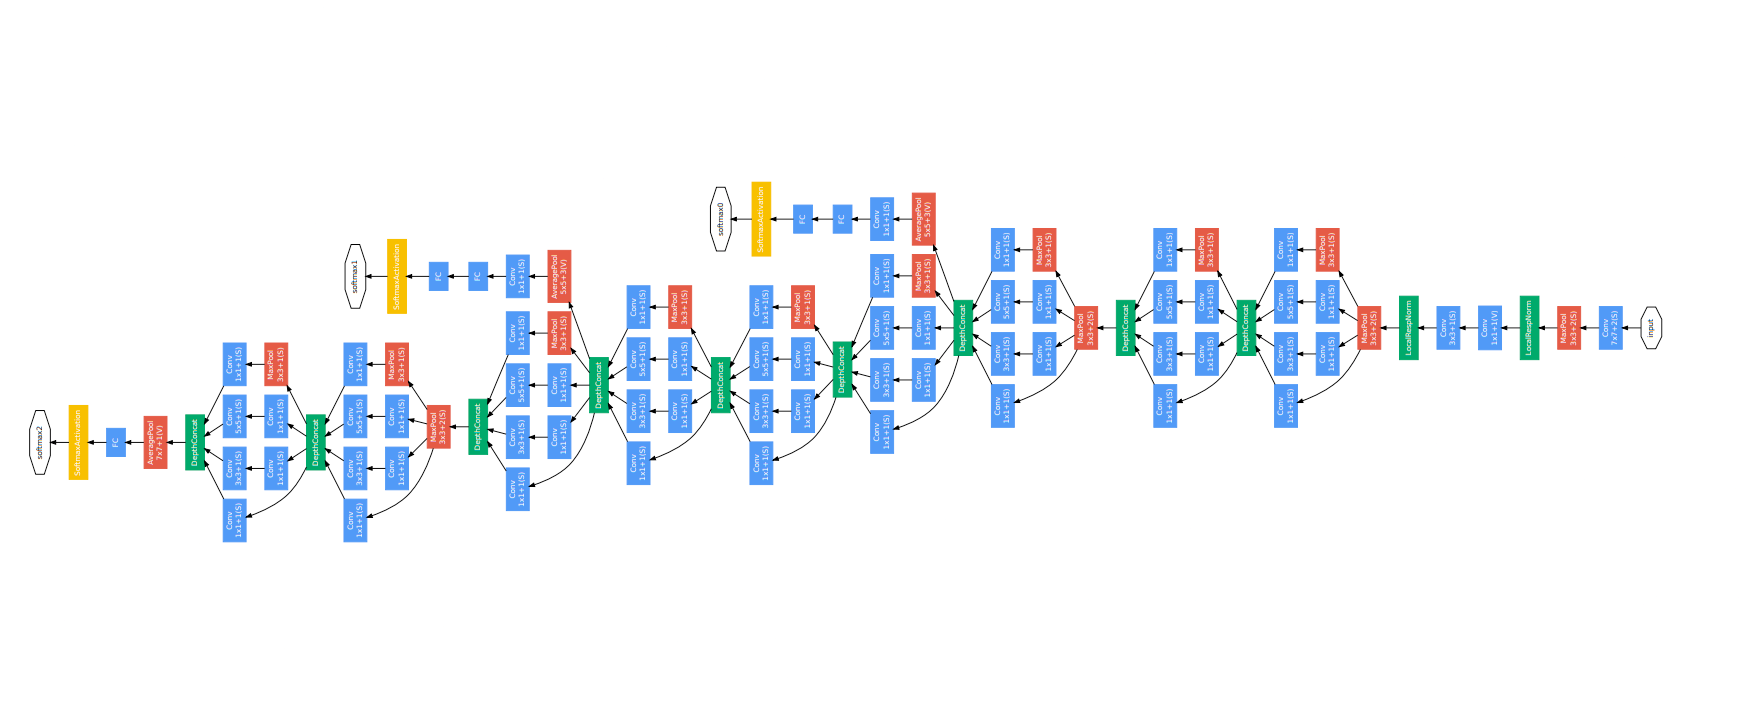
\includegraphics[width=0.99\linewidth]{./img/googlenet.png}
  \caption{GoogLeNet architecture}
\end{figure}

The network is composed by stem layers which shrink the image size, a stack of inception modules where a combination of different operations are combined, and a final classifier.
There are 22 trainable layers and about 100 modules (the blue and red blocks).

\paragraph{Stem layers}
Stem layers aggressively downsamples inputs: from 224 to 28 width/height in 5 layers.
It brings it down a bit more gently than AlexNet.
To reach $28\times 28$, VGG uses 10 layers.

\paragraph{Naïve inception module}
The main idea of the inception module is that it consists of multiple pooling and convolution operations with different sizes ($3\times 3$, $5\times 5$) in parallel, instead of using just one filter of a single size.
\begin{figure}[htbp]
  \centering
  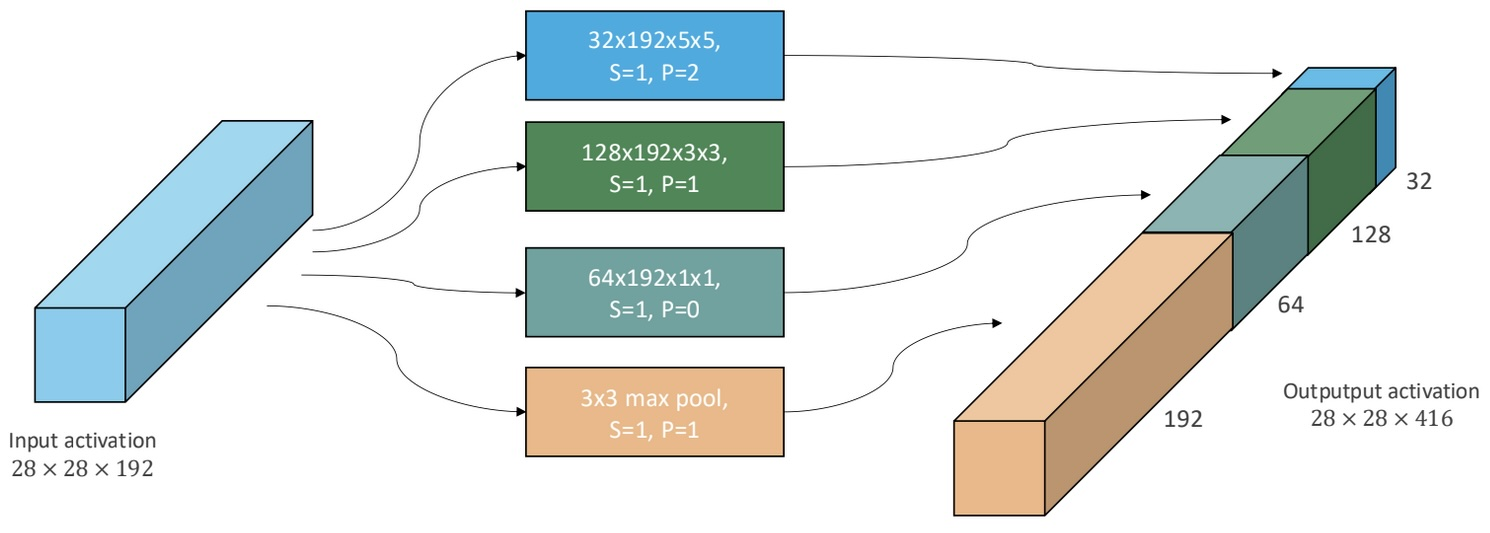
\includegraphics[width=0.8\linewidth]{./img/inception_naive.jpg}
  % \caption{}
\end{figure}
However, there are two main problems:
\begin{itemize}
  \item Due to max-pool, the number of channels grows very fast when inception modules are stacked on top of each other.
  \item $5 \times 5$ and $3 \times 3$ convolutions on many channels become prohibitively expensive if we stack a lot of them.
\end{itemize}

\paragraph{$1 \times 1$ convolutions and the inception module}
To overcome the problems, we use $1 \times 1$ convolutions before feeding the data into $3\times 3$ or $5 \times 5$ convolutions.
$1\times 1$ convolutions don't reason locally, but along the channel on a single dimension.
They allow us to change the depth of the activations while preserving the spatial size.
This is effectively a dimensionality reduction.

\begin{figure}[htbp]
  \centering
  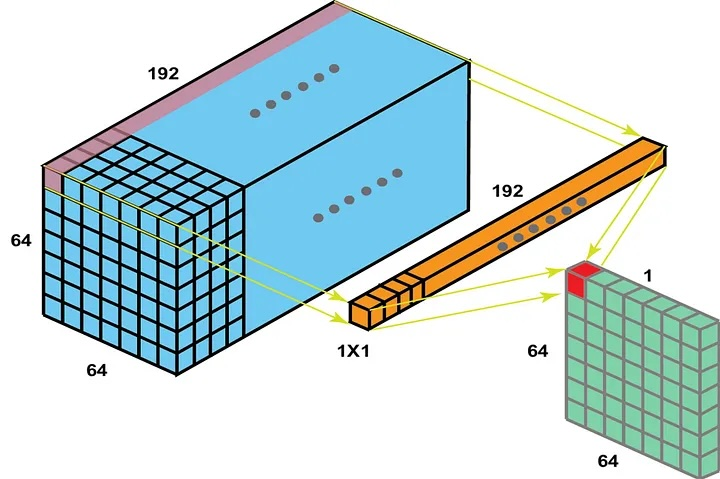
\includegraphics[width=0.8\linewidth]{./img/11conv.jpg}
  \caption{$1 \times 1$ convolution}
\end{figure}

By adding $1\times 1$ convolutions before larger convs and after max pool we can:
\begin{itemize}
  \item \textbf{Control the time complexity} of the larger convolutions by reducing the channel dimension.
  \item \textbf{Control the number of output channels} by reducing the depth of the max pool output.
\end{itemize}

\begin{figure}[htbp]
  \centering
  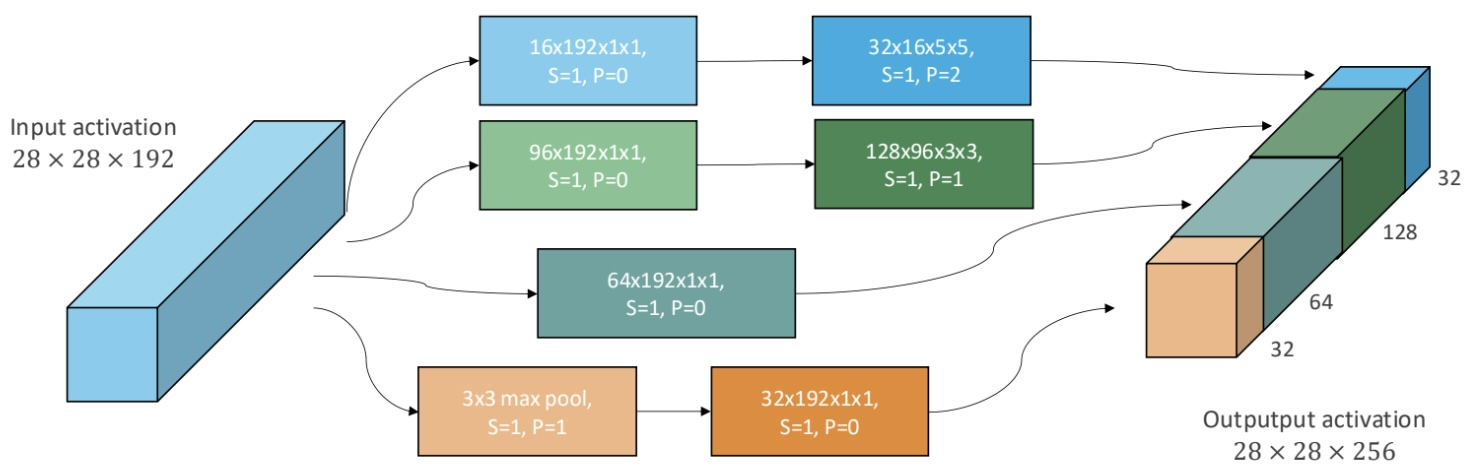
\includegraphics[width=0.8\linewidth]{./img/inception.jpg}
  \caption{Inception module in GoogLeNet}
  \label{fig:inception}
\end{figure}

In \ref{fig:inception} we can see how Google exploited the properties of $1\times 1$ convolutions to make an incpetion module without making the complexity explode.
The idea is that we take our input, we shrink it by using $1\times 1$ convolutions, and then we apply the $5 \times 5$ and $3 \times 3$ spatial convolutions.
We use $1\times 1$ convolutions \textbf{after} pooling to shrink the output (we don't need to compress before the operation but after it).

\paragraph{Fully-connected classifier vs global average pooling}
As we have seen the last 3 fully connected layers were the heaviest, since we had very high dimensional spatial information.
To reduce the number of parameters needed between convolutional features and fully connected layers we get rid of spatial dimensions by averaging them out, because the activations should contain high level information.

\subsubsection{Inception v3}
Inception v3 leverages convolution factorizations to increase the computational efficiency and to reduce the number of parameters, the two main methods are:
\begin{itemize}
  \item $3 \times 3$ followed by $3 \times 3$ instead of a $5 \times 5$ (VGG idea).
  \item $3 \times 3$ can be factorized in a $3\times 1$ and $1 \times 3$.
\end{itemize}

\begin{figure}[htbp]
  \centering
  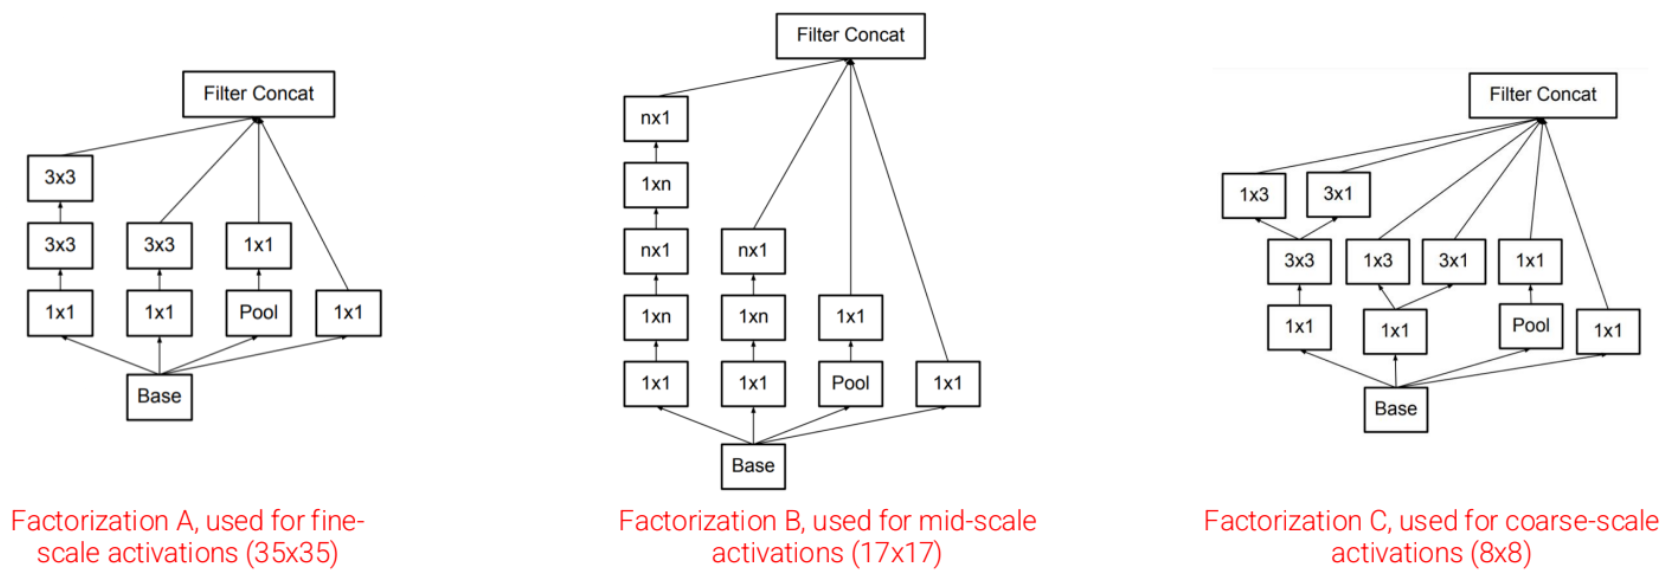
\includegraphics[width=0.8\linewidth]{./img/inception3.png}
  \caption{Instead of always using the same inception layers, we use 3 different inception layers}
\end{figure}

\subsubsection{Residual Networks (ResNet)}
ResNet was invented to address the problem of vanishing gradients and degradation in very deep neural networks.
The core innovation in ResNet is the residual block, which introduces skip connections.
In traditional networks, each layer feeds directly into the next layer.
In ResNet, the input to a layer is also added to its output, by creating what's called a skip connection (like an identity shortcut).
This means that instead of learning a direct mapping $H(x)$, the network learns the residual function $F(x) = H(x) - x$.

\begin{figure}[htbp]
  \centering
  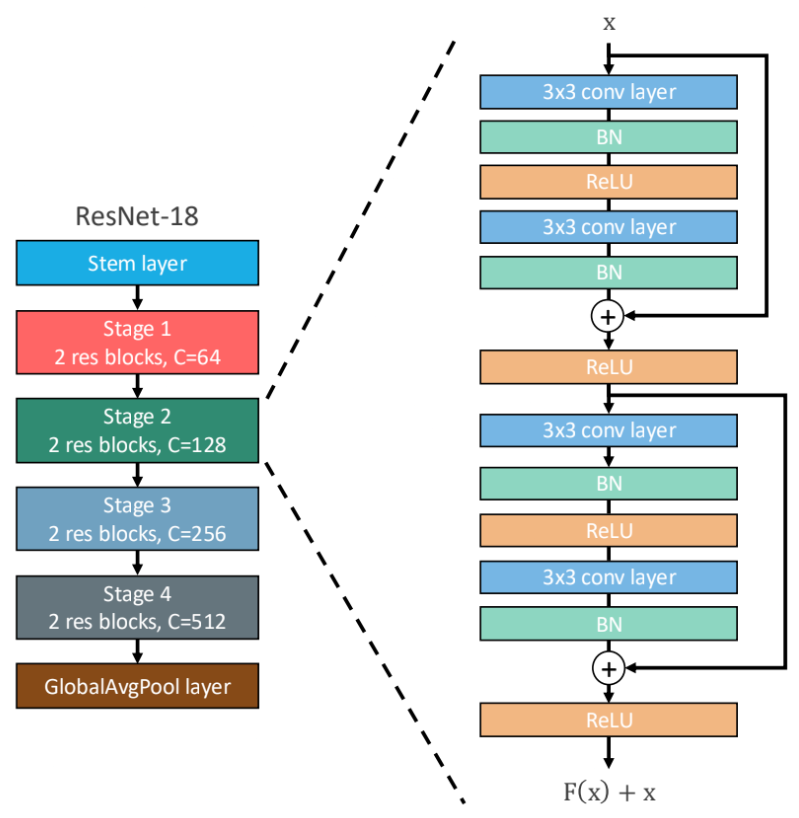
\includegraphics[width=0.8\linewidth]{./img/resnet.png}
  \caption{The ResNet architecture}
\end{figure}

The network is a stack of stages with fixed design rules (inspired by VGG):
\begin{itemize}
  \item Stages are a stack of residual blocks.
  \item Each residual block is a stack of two $3 \times 3$ convolutions with batch-norm.
  \item The first block of each stage halves the spatial resolution (with stride 2 convolutions) and doubles the number of channels.
  \item It uses stem layer and global average pooling as GoogLeNet.
\end{itemize}

\begin{figure}[htbp]
  \centering
  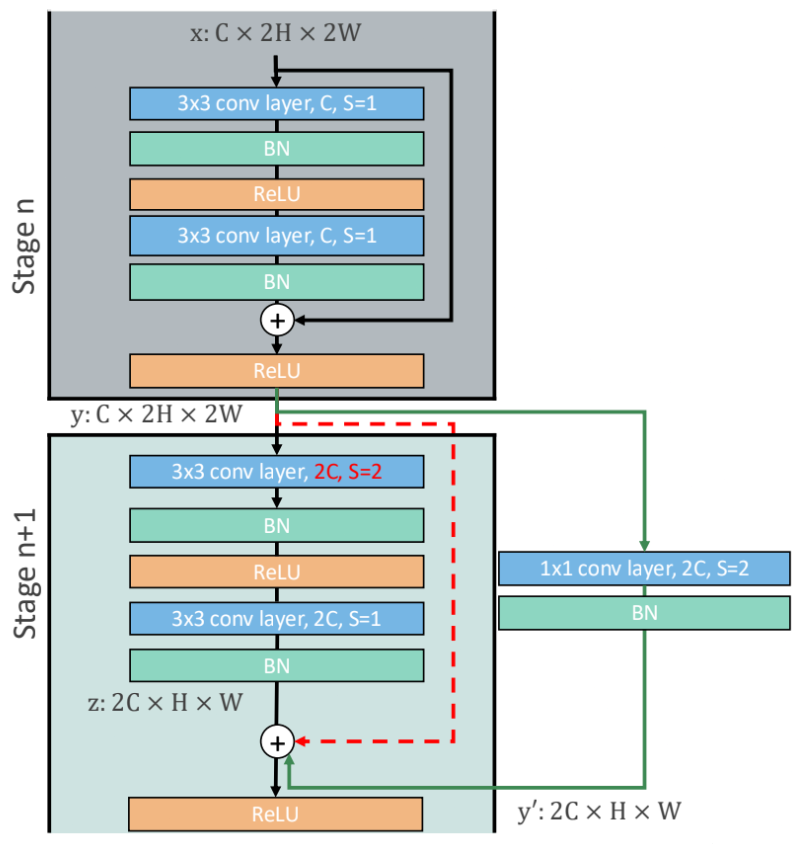
\includegraphics[width=0.8\linewidth]{./img/resnet_skip.png}
  % \caption{}
\end{figure}

ResNet is still the standard baseline for most tasks today.

The residual blocks described so far \textbf{cannot be used as the first block of a new stage}, because the number of channels and the spatial dimensions do not match along the residual connection.
The authors then decided to use a $1\times 1$ convolution with stride 2 and $2C$ output channels to expand the dimension of the channels.

\paragraph{Bottleneck residual block}
A bottleneck residual block is a design used in very deep ResNets (e.g. ResNet-50, 101, 152) to enable training with more layers while maintaining computational efficiency.
\begin{figure}[htbp]
  \centering
  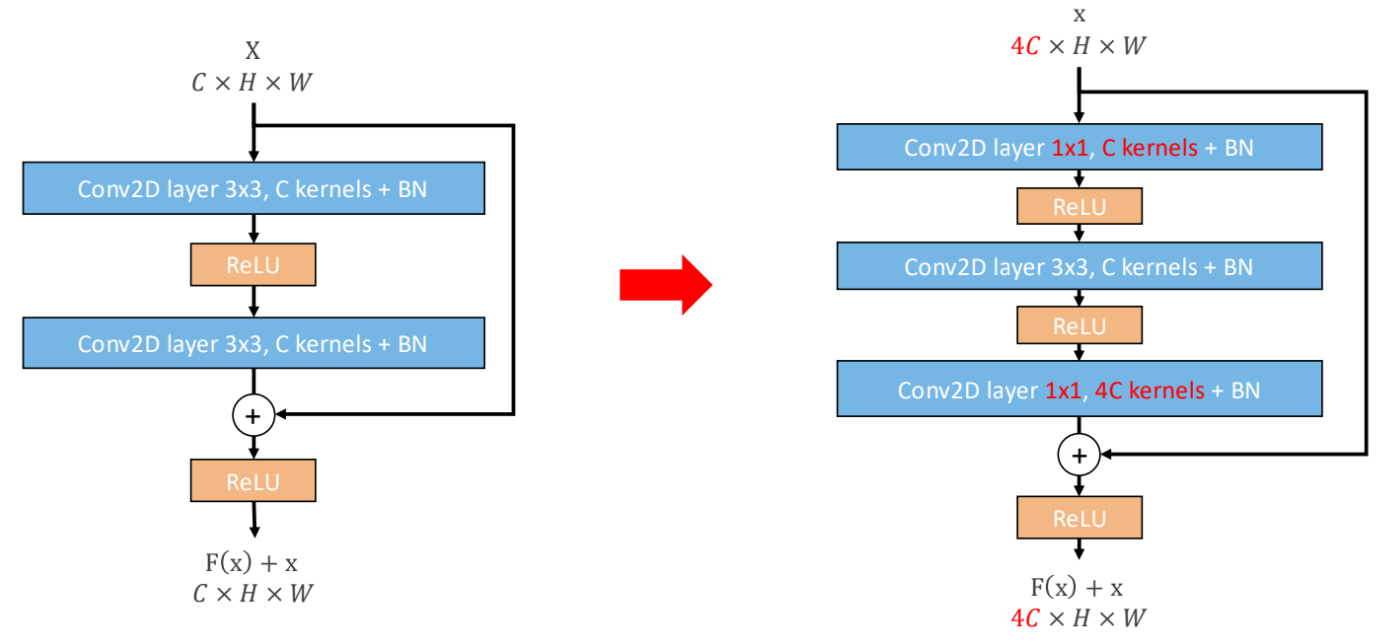
\includegraphics[width=0.8\linewidth]{./img/resnet_bottleneck.png}
  \caption{Instead of working with $3 \times 3$ convolutions we go from $4C$ down to $C$ and then expand again}
\end{figure}

\subsubsection{ResNeXt}
Inception modules are effective multi-branch architectures, which can be thought of as following a split-transform-merge paradigm.
ResNeXt is a simpler way to realize multiple pathways, since it decomposes each bottleneck residual block of ResNets into $G$ parallel branches.
The number of branches (cardinality) is a new hyperparameter.
Once $G$ is chosen, it is possible to obtain a $G \times d$ ResNeXt block with complexity similar to the original ResNet block.
$d$ must be proportional to $C$.

\paragraph{ResNeXt block as grouped convolutions}

Grouped convolutions split input channels into $G$ independent groups.
Each group processes a subset of channels, reducing computational cost and parameters while maintaining feature diversity.

\begin{figure}[htbp]
  \centering
  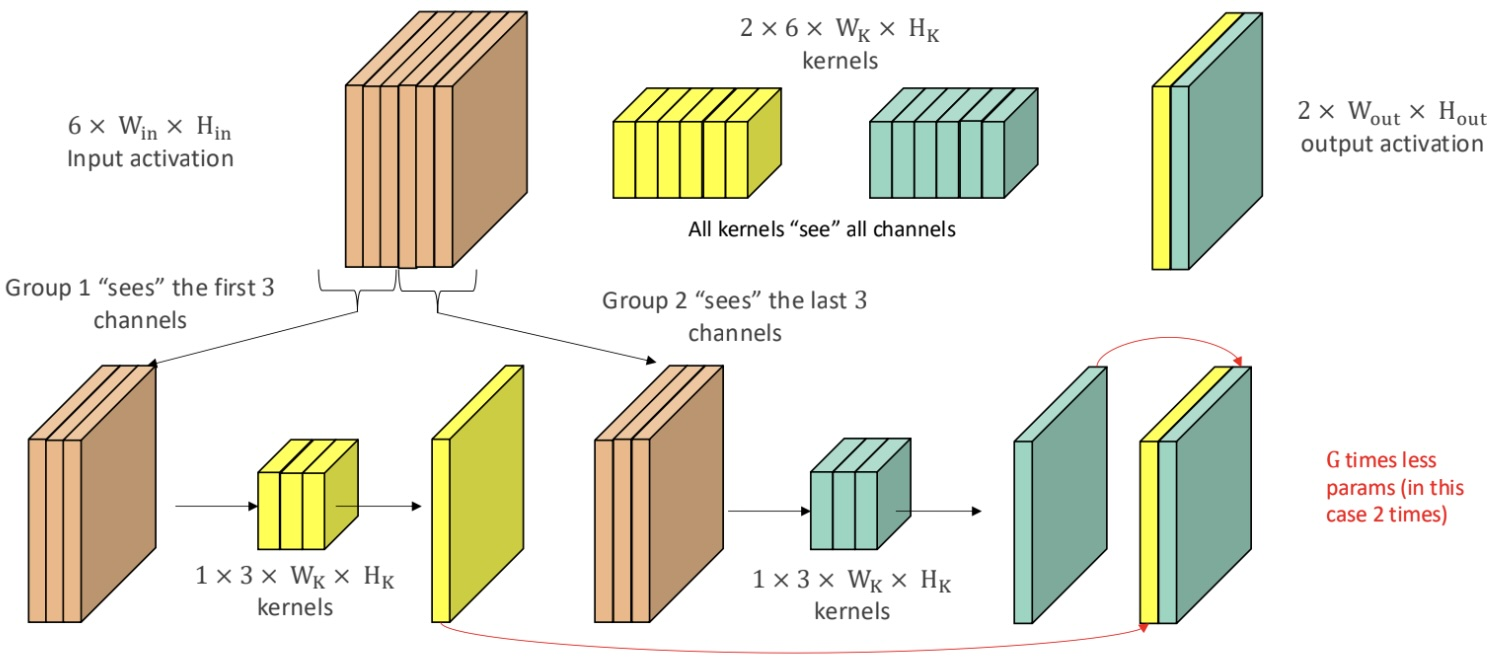
\includegraphics[width=0.8\linewidth]{./img/grouped_convolutions.jpg}
  \caption{Grouped convolution with $G=2$}
\end{figure}

An input with $C$ channels is divided into $G$ groups, each with $\frac{C}{G}$ channels.
Each group has its own filters, producing $\frac{K}{G}$ output channels (for $K$ total filters).
The outputs are concatenated, resulting in $K$ channels.

This is useful because it's more efficient and each group learns distinct features, enhancing model capacity.

ResNeXt introduces cardinality (the number of groups of $G$) as a new dimension.
It uses grouped convolutions to create parallel pathways within a residual block, improving feature learning without increasing depth/width.

\begin{figure}[htbp]
  \centering
  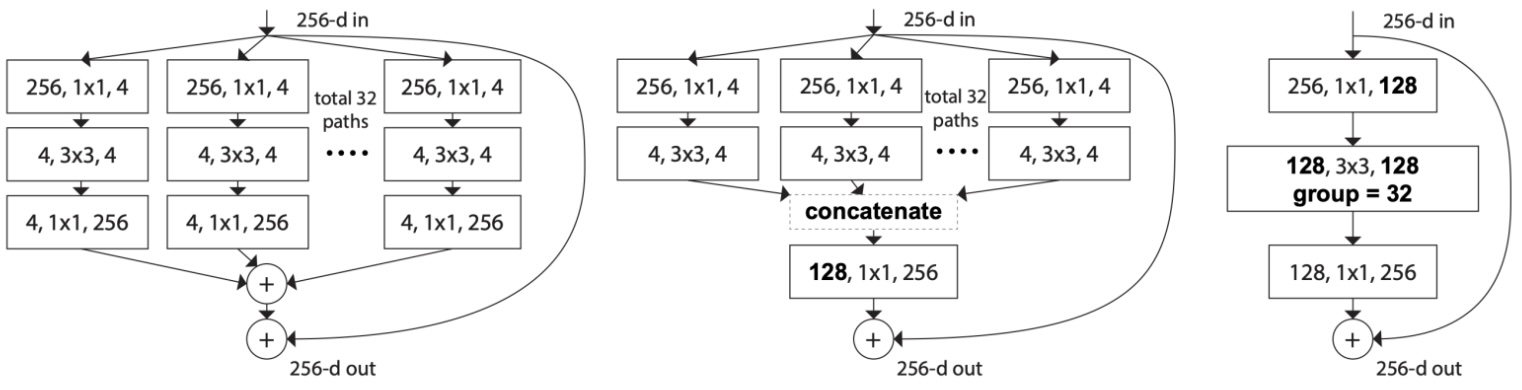
\includegraphics[width=0.8\linewidth]{./img/resnext_grouped.jpg}
  \caption{The ResNeXt block as grouped convolutions, on the left we have a normal convolutional block, in the middle we split to reduce computation and on the right we join again.}
\end{figure}

The structure of the ResNeXt block is:
\begin{itemize}
  \item $1\times 1$ convolution to compress the input channels.
  \item $3\times 3$ grouped convoltuion to process compressed features in $G$ parallel groups (cardinality). Each group applies transformations independently.
  \item $1\times 1$ convolutions expands channels back.
  \item skip connection adds the original input to the output (residual learning).
\end{itemize}

ResNeXt is more efficient because there are fewer parameters than widening/deepening the network, and by increasing $G$ we can improve the performance without drastically increasing the compute.

\subsubsection{Squeeze-and-Excitation Networks (SENet)}
It's the last paper which won CVPR.
It proposed the squeeze-and-excitation module to capture global context and to use it to reweight channels in each block.
Given the output $U$ of a block with shape $C \times H \times W$ we do:
\begin{itemize}
  \item Global average pooling to squeeze.
  \item General bottleneck formed by two fully connected layers with reduction ratio 16.
\end{itemize}

\begin{figure}[htbp]
  \centering
  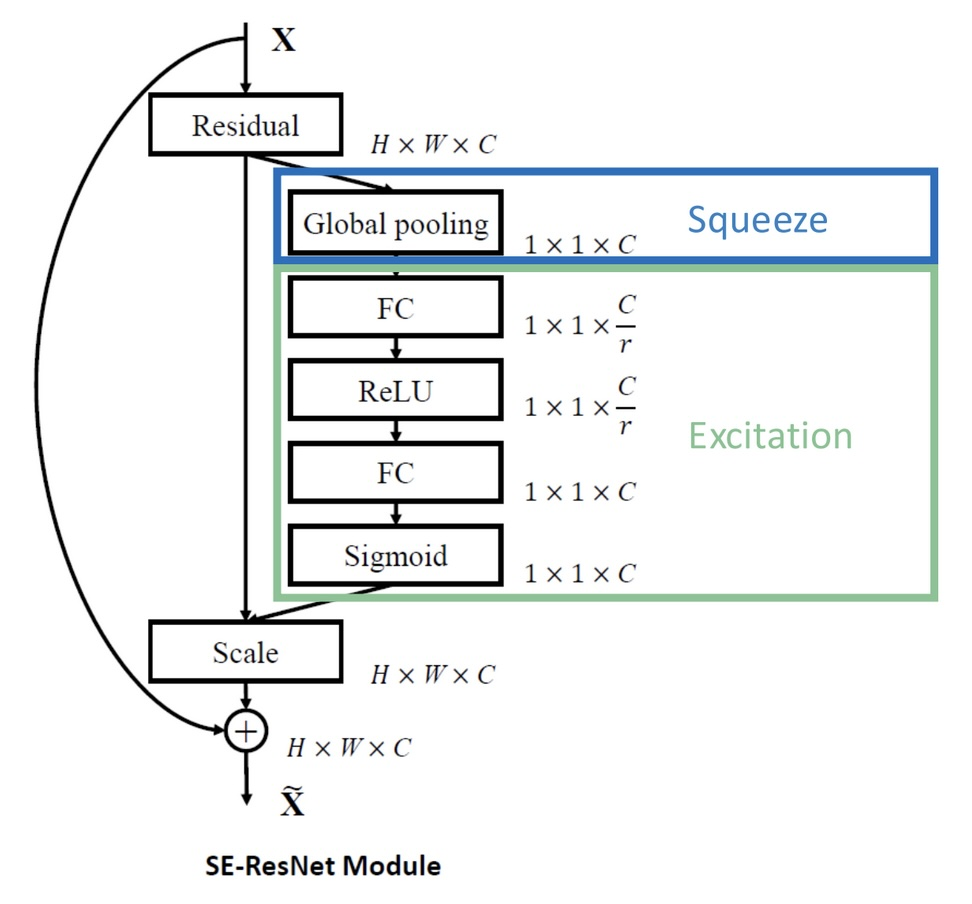
\includegraphics[width=0.8\linewidth]{./img/senet.jpg}
  \caption{SENet block diagram}
\end{figure}

\subsubsection{Depthwise Separable convolutions}
F. Chollet one year after the SENet paper proposed the Depthwise Separable convolutions.
The standard convolutions filter features based on the convolutional kernels and combine features in order to produce new representations.
This is very expensive.
Depthwise separable convolutions separates filtering and combination, and this aggressively limits the computational cost.

\begin{figure}[htbp]
  \centering
  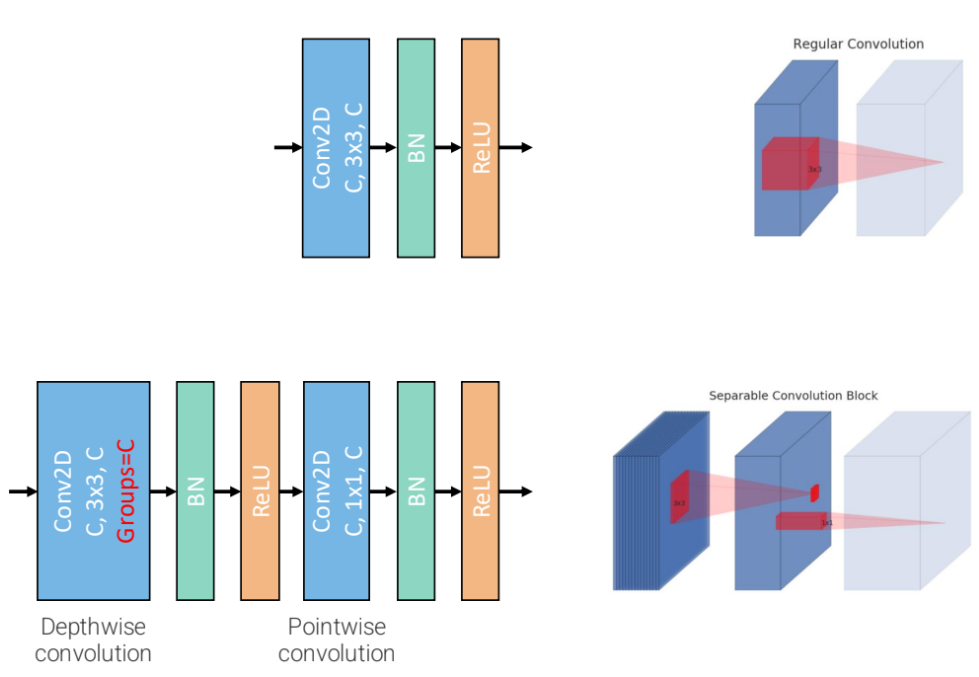
\includegraphics[width=0.8\linewidth]{./img/separable_convolution.png}
  % \caption{}
\end{figure}

\subsubsection{Inverted residual blocks}
MobileNet-v2 introduced the bottleneck residual block to scale up the model depth by increasing the number of layers per block while keeping the computation and number of parameters roughly constant.
To this end, it uses a pair of $1\times 1$ convolutions, where the first compresses the number of channels, while the second one expands them.
Hence, the $3\times 3$ convoltuion operates in the compressed domain.

\begin{figure}[htbp]
  \centering
  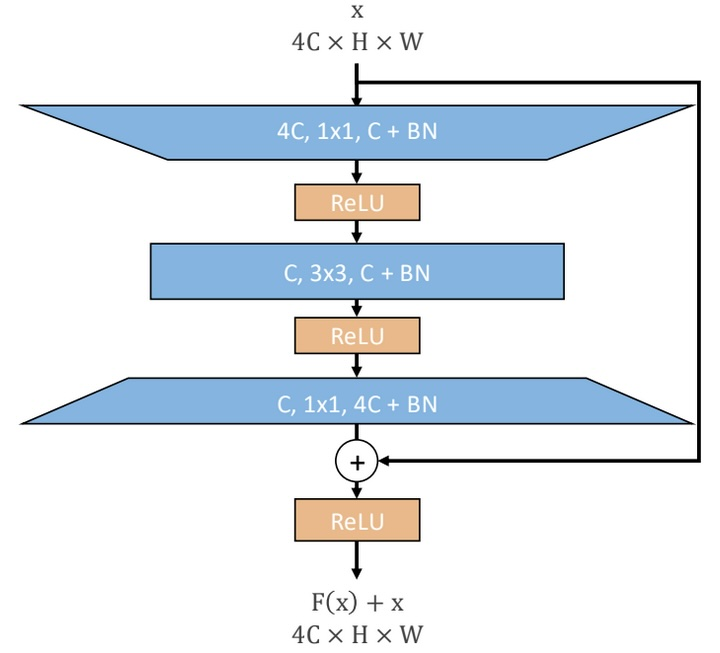
\includegraphics[width=0.8\linewidth]{./img/bottleneck_residual.jpg}
  % \caption{}
\end{figure}

As we know, compression usually results in information loss, so in MobileNet-v2 inverted residual blocks were proposed.
In this blocks, the first $1\times 1$ convolution expands the channels, while the second compresses them back, according to an expansion ratio $t$.
To limit the increase in computation, the inner $3\times 3$ convolution is realized as a depthwise convolution (single filter per input channel instead of applying the filters across all the input channels).

\begin{figure}[htbp]
  \centering
  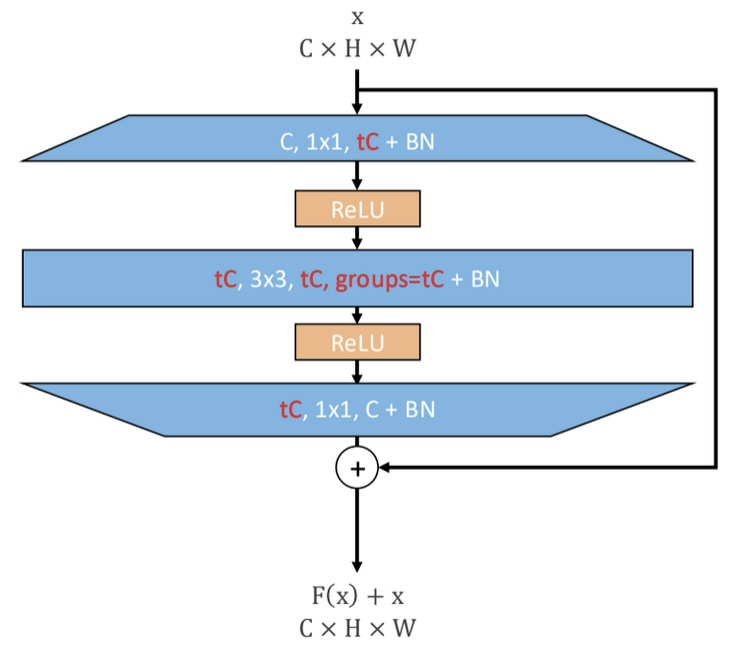
\includegraphics[width=0.8\linewidth]{./img/inverted_residual.jpg}
  % \caption{}
\end{figure}

\subsubsection{MobileNet-v2}
MobileNet-v2 is a stack of inverted residual blocks with ReLUs in between.
The number of channels grows slowly compared to previous architectures, as we can see in the purple rectangle in figure \ref{fig:mobilenet}

\begin{figure}[htbp]
  \centering
  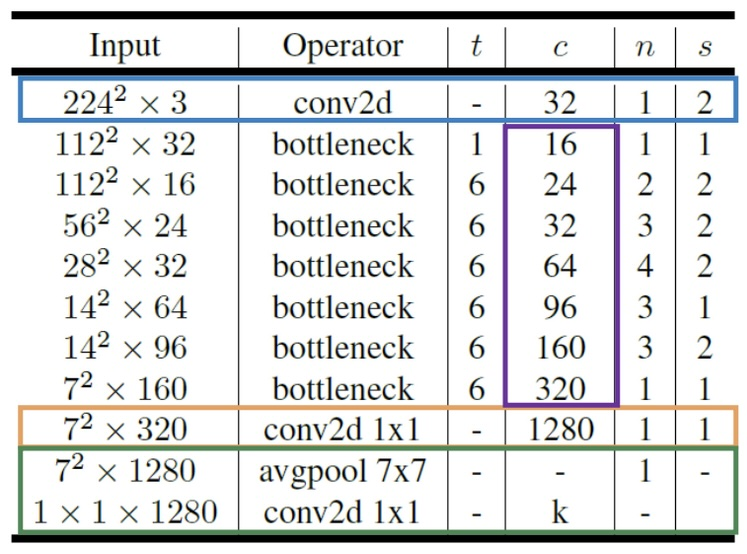
\includegraphics[width=0.8\linewidth]{./img/mobilenet.jpg}
  % \caption{}
  \label{ref:mobilenet}
\end{figure}

Whenever spatial dimensions or number of channels do not match between input and output, there are no residual connections.

\subsubsection{EfficientNet}
EfficientNet proposed to design the network based on resources.
As we know there are 3 dimensions for scaling a neural network: width, depth and resolution.

\begin{figure}[htbp]
  \centering
  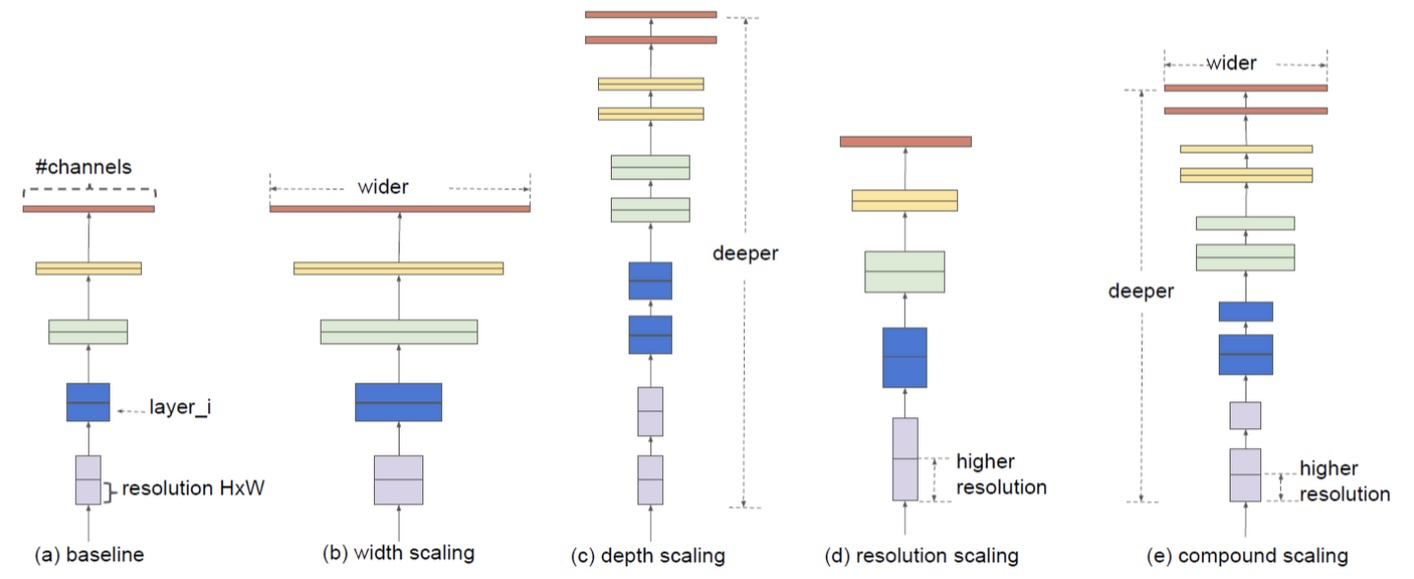
\includegraphics[width=0.8\linewidth]{./img/efficientnet.jpg}
  \caption{Different types of NN scaling.}
\end{figure}

Bigger networks with larger width, depth or resolution tend to achieve higher accuracy, but the accuracy gain quickly saturates after reaching $80 \%$, which is a limitation of single dimenison scaling.
\textbf{Scaling dimensions are not independent}. Intuitively, for higher resolution images, we should increase network depth, such that the larger receptive fields can help to capture similar features that include more pixels in bigger images.
Correspondingly, we should also increase netowrk width when the network resolution is higher, in order to capture more fine-grained patterns with more pixels in high resolution images.

EfficientNet  uses a compound coefficient $\phi$ to scale all dimensions in a principled way.

\subsection{RNNs \& Transformers}

In RNNs, which were used to avoid the problem of fixed size input, the gradient computetion involves performing a forward propagation pass moving from left to right through the unrolled graph of the network, followed by a backward propagation pass moving right to left through the graph.
The basic problem is that by propagating the gradient over many stages it tends to vanish or explode, so learning long-term dependencies can take a lot of time.

\paragraph{Encoder-Decoder architecture}
In this type of architecture the encoder processes the input sequence.
It emits the context $C$, usually as a function of its final hidden state.
The decoder is conditioned on that fixed-length vector to generate the output sequence.
If the context $C$ is a vector, then the encoder RNN is simply a sequence-to-vector RNN, and the decoder is a vector-to-sequence RNN.
The \textbf{bottleneck problem} arises because the context $C$ outputted by the encoder RNN has a dimension that is too small to properly summarize a long sequence.

\paragraph{Attention}
Existing model for neural machine translation encode a source sentence into a fixed-length vector from which a decoder generates a translation.
Attention provides a solution to the bottleneck problem. 
We provide to the decoder the learned token start, then we do the dot product between the start token and the hidden states.
All the other hidden states give us a probability for each token.

\begin{figure}[htbp]
  \centering
  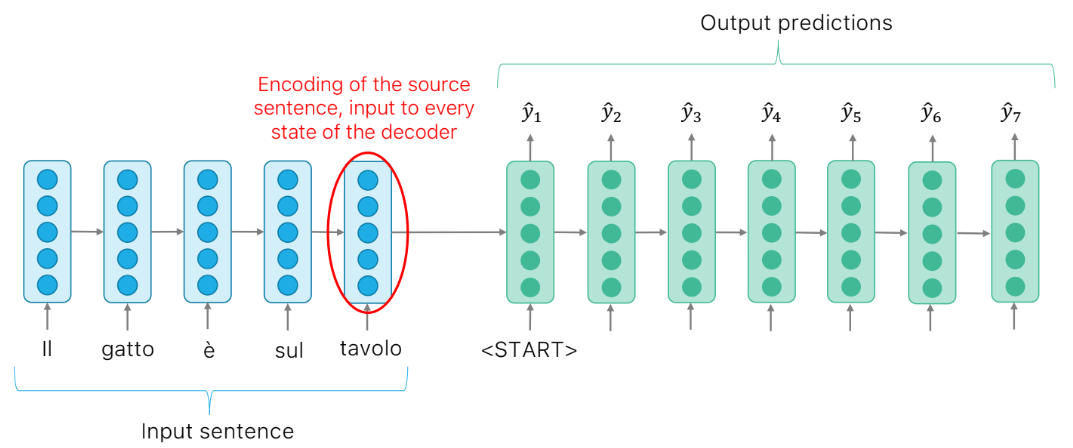
\includegraphics[width=0.8\linewidth]{./img/rnn_classic.png}
  \caption{In the classic RNN, the last hidden state is used for all the translation.}
\end{figure}

\begin{figure}[htbp]
  \centering
  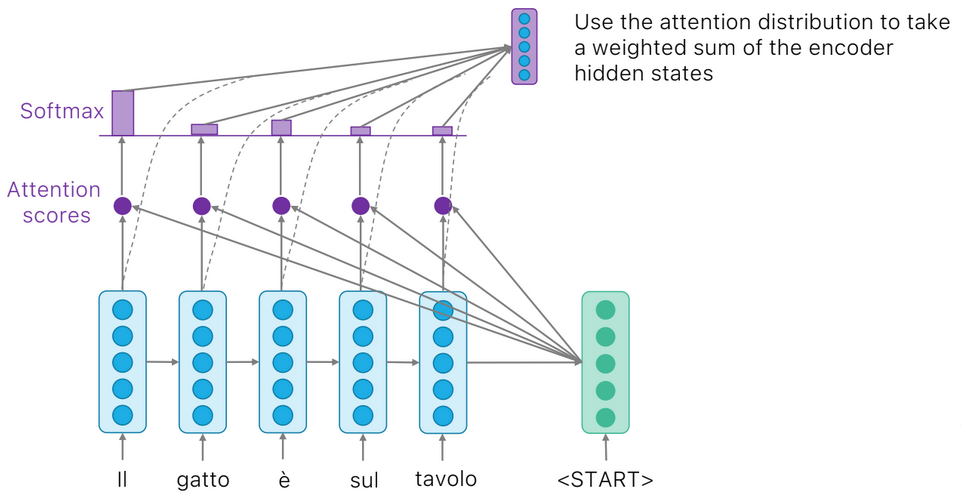
\includegraphics[width=0.8\linewidth]{./img/attention.png}
  \caption{In the attention mechanism, at each step, the current hidden state is compared with all the previous hidden states by computing an attention score.}
\end{figure}

\subsubsection{Transformer architecture}
The inherently sequential nature of RNN precludes parallelization within training examples, which becomes critical with longer sequence lengths.
The \textbf{transformer} is the first model relying entirely on self-attention (and cross-attention) to compute representations of its input and output without using RNNs or convolutions.
It's still an encoder-decoder architecture, where the encoder maps an input sequence of symbol representations $(x_1, ..., x_n)$ to a sequence of continuous representations $z=(z_1, ..., z_n)$.
Given $z$, the decoder generates an output sequence $(y_1, ..., y_m)$ of symbols one element at a time.
At each step the model is \textbf{auto-regressive}, consuming the previously generated symbols as additional input when generating the next.

\begin{figure}[htbp]
  \centering
  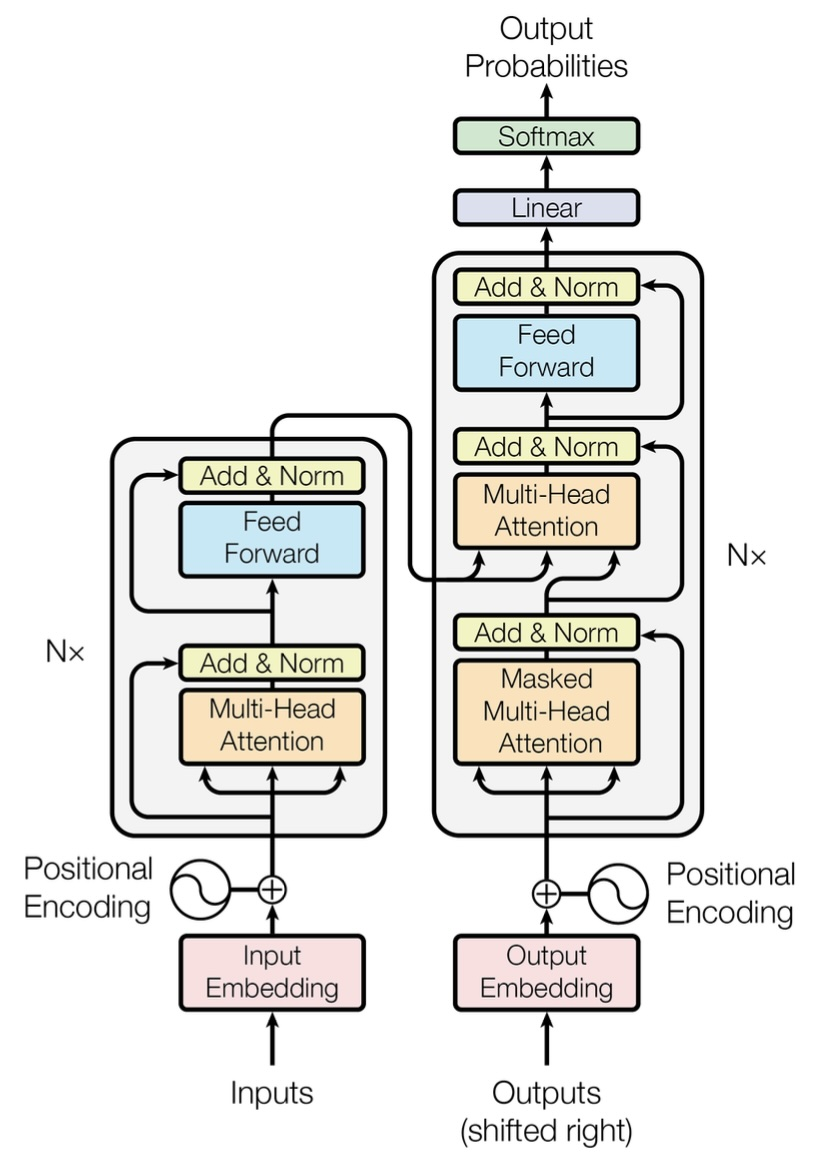
\includegraphics[width=0.6\linewidth]{./img/transformer.jpg}
  \caption{The transformer architecture from the paper "Attention is all you need".}
\end{figure}

\paragraph{Transformer encoder}
In the encoder we turn each input word into a vector by using an embedding layer.
Each word is embedded into a vector of size $d_{\text{model}}$.
If the encoders are stacked, the embedding only happens in the bottom-most encoder.
Since we process the words in parallel we lose positional information, so by using positional encoding we keep this information.
The positional encoding has the same dimension $d_{\text{model}}$ as the embeddings, so that the two can be summed.
There are learned and fixed positional encodings; the authors used sine and cosine functions of different frequencies.

Each layer has two sub-layers:
\begin{itemize}
  \item A multi-head self attention mechanism.
  \item A fully connected feed-forward network. The exact same feedforward network is independently applied to each position (shared parameters).
\end{itemize}

There is also a residual connection around each of the two sub-layers, followed by layer normalization.
To facilitate these residual connections, all sub-layers in the model, as well as the embedding layers, produce outputs of dimension $d_{\text{model}}$.

\paragraph{Transfromer decoder}
The decoder is also composed of a stack of $N$ identical layers.
In addition of the two sub-layers of the encoder, the decoder has a third sub-layer, which performs multi-head attention over the output of the encoder stack (cross-attention).
As in the encoder tehre are residual connections and layer normalization.

The self-attention sub-layer in the decoder stack is modified so as to \textbf{prevent positions from attending to subsequent positions}.
This masking, combined with the fact that the output embeddings are offset by one position, ensures that the predictions for position $i$ can depend only on the known outputs at positions less than $i$.

\paragraph{Self-Attention}
The first setp in calculating self-attention is to create three vectors from each of the embedded words:
\begin{itemize}
  \item a Query vector.
  \item a Key vector.
  \item a Value vector.
\end{itemize}

These vectors are created by multiplying the embeddings by three matrices learned during the training process.
Their dimensionality is $d_k = \frac{d_{\text{model}}}{h}$, while the embedding and encoder input/output vectors have dimensionality of $d_{\text{model}}$.

The matrices are used to compute the self-attention score.
$$\text{Attention}(Q,K,V)=\text{softmax}(\frac{QK^T}{\sqrt{d_k}})V$$

As we can see there is a little normalization done with $\sqrt{d_k}$, to try to avoid having the results of the softmax squeezed too much into a single value (one hot).
The scores of the self-attention determine how much focus to place on other parts of the input sentence as we encode a word at a certain position.

\paragraph{MultiHead Attention}
The purpose of multi-head attention is to linearly project the queries, keys and values $h$ times with different, learned linear projections.
On each of these projected versions of queries, keys, and values we perform the attention function in parallel.
The outputs of different heads are then concatenated and once again projected.
Multi-head attention allows the model to jointly attend to information from different representation subspaces at different positions.

\paragraph{Multi Head Self-Attention computation}

\paragraph{Cross-Attention}
in the cross attention layers, the queries come from the previous decoder layer (masked self-attention), and the keys and values come from the output of the encoder.
This allows every position in the decoder to attend over all positions in the input sequence.
It's a very powerful mechanism used in modern generative models to introduce variable lengths conditions.


\subsubsection{Vision Transformer (ViT)}
We split an image into patches and provide the sequence of linear embeddings of these patches as an input to a Transformer.
The image patches are treated the same way as tokens in an NLP application.

As an alternative to raw image patches, the input sequence can be formed from feature maps of a CNN.
In this hybrid model, the patch embedding projection is applied to patches extracted from a CNN feature map.

To handle $2D$ images, we reshape the image $x \in \mathbb{R}^{H\times W \times C}$ into a sequence of flattened $2D$ patches $x_p \in \mathbb{R}^{N \times (P^2 \cdot C)}$.
\begin{itemize}
  \item $(H, W)$ is the resolution of the original image.
  \item $C$ is the number of channels.
  \item $(P, P)$ is the resolution of each image patch.
  \item $N = \frac{HW}{P^2}$ is the resulting number of patches, which also serves as the effective input sequence length for the transformer.
\end{itemize}

The transformer uses constant latent vector size $d_{\text{model}}$ through all of its layers, so we flatten the patches and map to $d_{\text{model}}$ dimensions with a trainable linear projection.
We also prepend a learnable embedding to the sequence of embedded patches, whose state at the output of the transfromer encoder serves as the image representation.
The classification head is implemented by a MLP with one hidden layer.
To retain positional information the ViT uses learnable 1D position embeddings.

At the start, the ViT worked very bad.
This is because transformers lack some of the inductive biases inherent to CNNs, such as translation equivariance and locality, and therefore do not generalize well when trained on insufficient amounts of data.
The convolution in combination with max pooling/striding makes CNNs approximately invariant to translation.
When a module is translation invariant, it means that if we apply translation transformation on the input image the output of the module won't change.
To solve the inductive bias they gave the network so much data that the classes appear anywhere.

\subsection{Object Detection}
Previously, we have done object detection with SIFT, but we were just able to say if the object was in the image, not where it was.
Now we want to do detection by putting a bounding box around the object.
We do this by returning a set of quadruples: $[x, y, h, w, o]_{i=0}^{K}$, where we have the box position, width, height, and class of the output.

The main challenges are the different lengths of the outputs (since we can detect from 0 to $K$ images), the fact that the outputs have both categorical and spatial information, and the fact that the images are usually processed at higher resolution than neural networks for image classification.

\subsubsection{Viola-Jones Object Detector}
It's a general purpose object detection framework, but it has been mainly applied to faces.
We will now see the three main innovations of the algorithm: the AdaBoost algorithm, cascade, and the use of integral images.

\paragraph{AdaBoost algorithm}
A Weak Learner (WL) is a simple classifier whose error is slightly better than random guessing.
Boosting is a way to train and build an ensemble of $M$ weak classifiers to obtain a Strong Learner SL.
After training a weak learner, the examples are re-weighted in order to emphasize those which were incorrectly classifier by the previous weak classifier.

The \textbf{AdaBoost} algorithm steps are:
\begin{enumerate}
  \item Given $N$ training samples $(x^(i), y^(i))$, assign equal weight to each training example $w^(i)=\frac{1}{N}$.
  \item Iterate for $j = 1, ..., M$ weak learners:
  \begin{enumerate}
    \item Fit the best classifier $WL_j$ to the training data by using the current weights.
    \item Compute the weighted error rate $\epsilon_j = \sum_{i:\, x^{(i)} \text{ is missclassified}} w^{(i)}$.
    \item Compute $\beta_j = \frac{1 - \epsilon_j}{\epsilon_j}$.
    \item Updates weights $w^(i) = w^(i)\beta_j$ for wrongly classified examples.
    \item Re-normalize $w^(i)$ to sum to 1.
  \end{enumerate}
  \item The Strong Learner is given by a weighted majority vote $SL(x) = \sum_{j} \ln \beta_j WL_j(x) > 0$, con $\ln \beta_j = \alpha_j$.
\end{enumerate}

The idea is that missclassified examples gain weight, forcing subsequent learners to focus on harder cases.

\paragraph{Haar-like features}
Weak classifiers used to detect faces are simple rectangular filters, composed of 2 to 4 rectangles applied at a fixed position within a $24 \times 24$ patch.
Even with this simple definition there are over $160$ k possible filters in a $24 \times 24$ patch.
AdaBoost is used to select a small subset of the most effective filters.

\paragraph{Dataset}
The dataset consisted of 4916 hand labeled faces, scaled and aligned to a base resolution of $24 \times 24$ pixels.
The non-face windows were collected by selecting random sub-windows from a set of 9500 images which did not contain faces.

\begin{figure}[htbp]
  \centering
  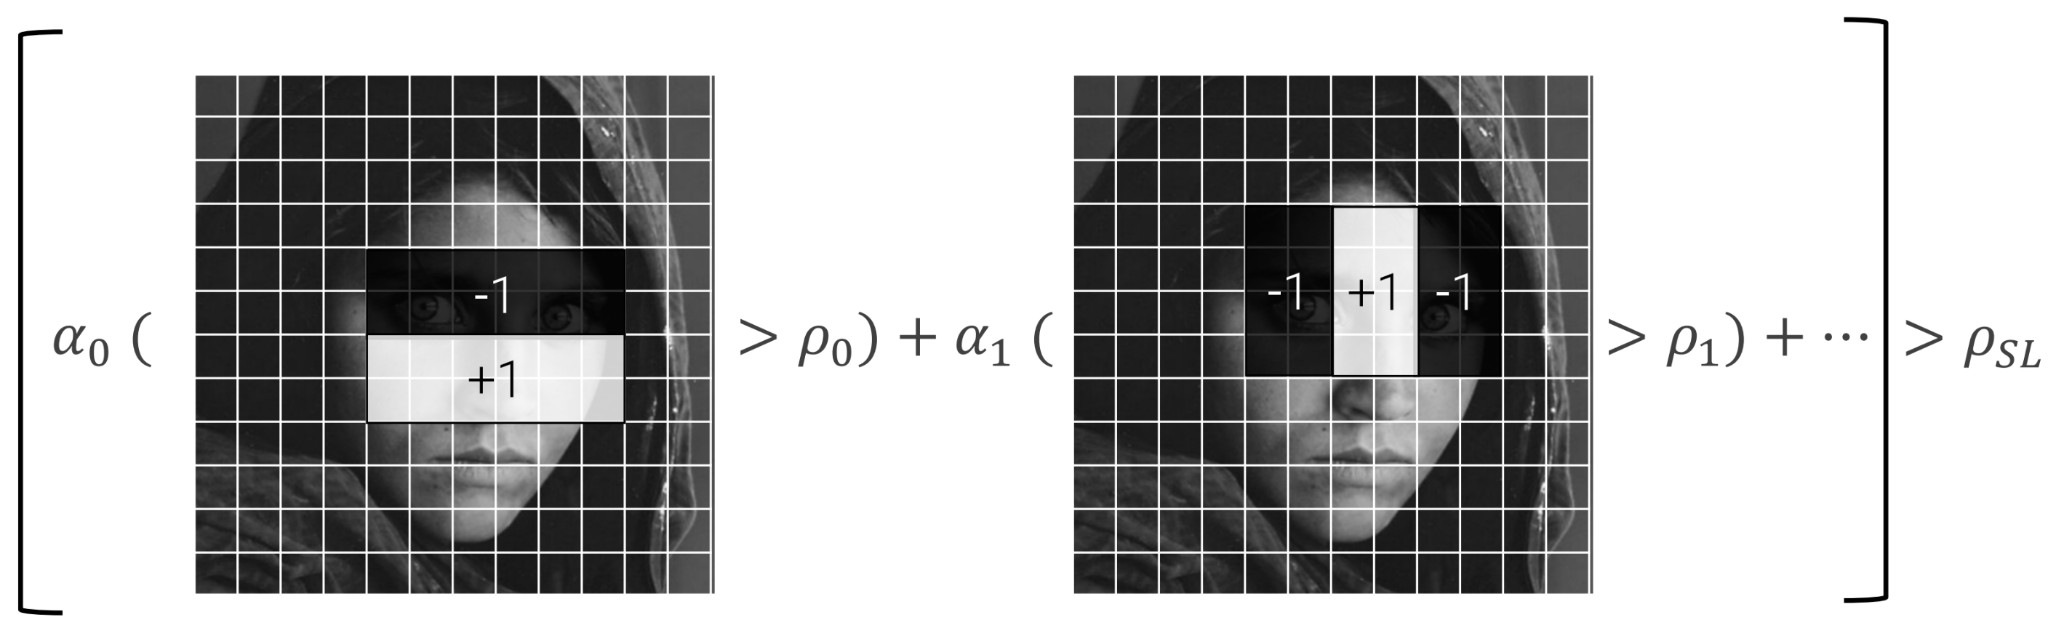
\includegraphics[width=0.6\linewidth]{./img/adaboost.png}
  \caption{The 2 most effective features selected by AdaBoost on the training set.}
\end{figure}

\paragraph{Integral images and fast feature computation}
To speed up the computation of rectangular features, the authors proposed the use of so-called integral images $II$, where $II(i,j) = \sum_{i' \leq i, j' \leq j} I(i', j')$.

We can compute the value of $II(i,j)$ just by looking at the 3 neighbours: $II(i,j) = II(i, j-1) + II(i-1, j) - II(i-1, j-1) + I(i,j)$, where $II$ are the values in the integral image, and $I$ is the value in the original image.

\begin{figure}[htbp]
  \centering
  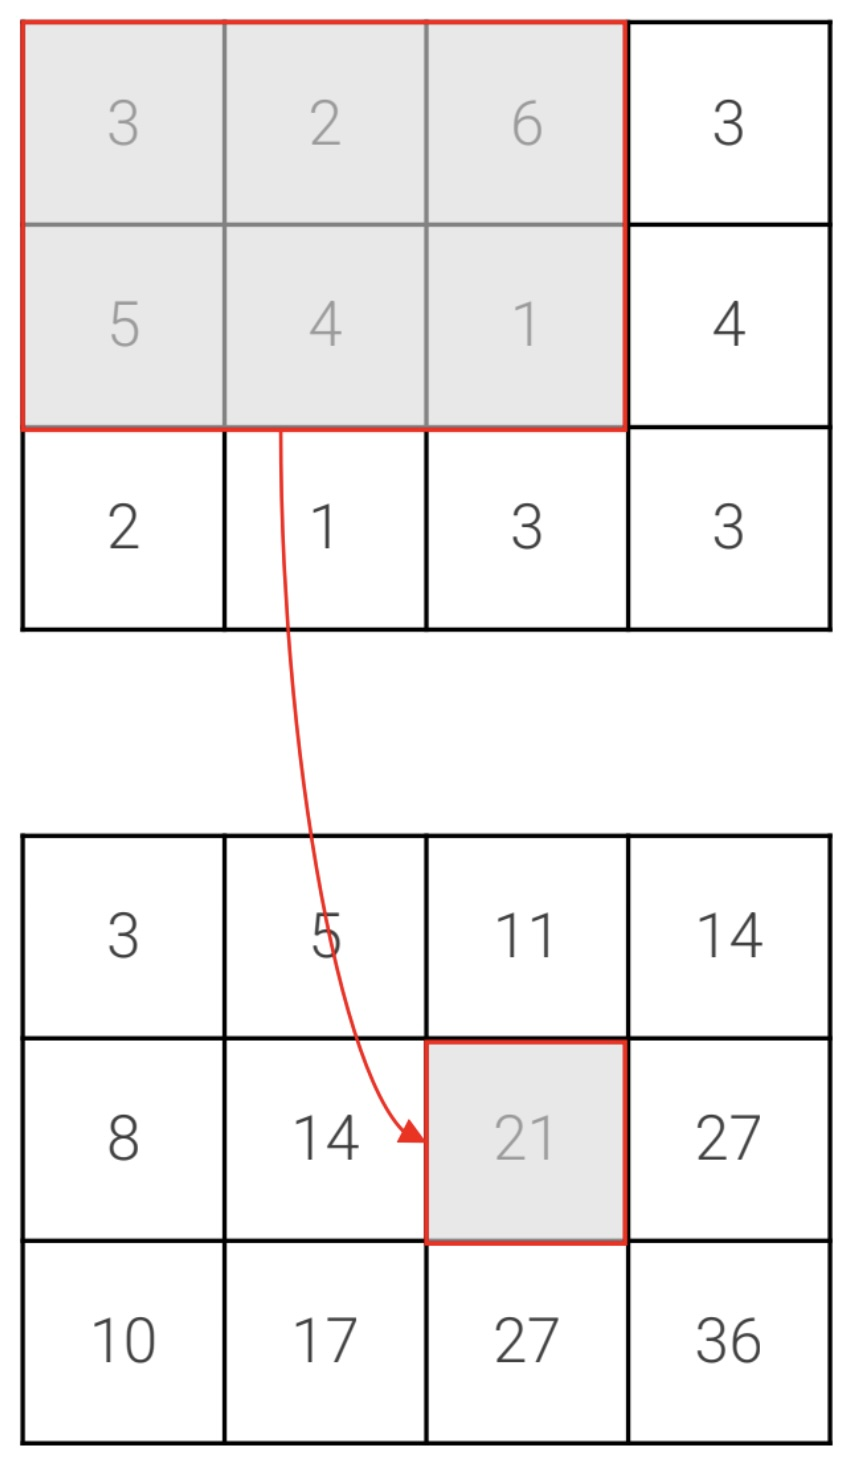
\includegraphics[width=0.6\linewidth]{./img/integral_images.jpg}
  \caption{$II(1,2) = II(1,1) + II(0,2) - II(0,1) + I(1,2) = 14 + 11 - 5 + 1$}
\end{figure}

With integral images we could have an overflow problem if numbers get too big.

\begin{figure}[htbp]
  \centering
  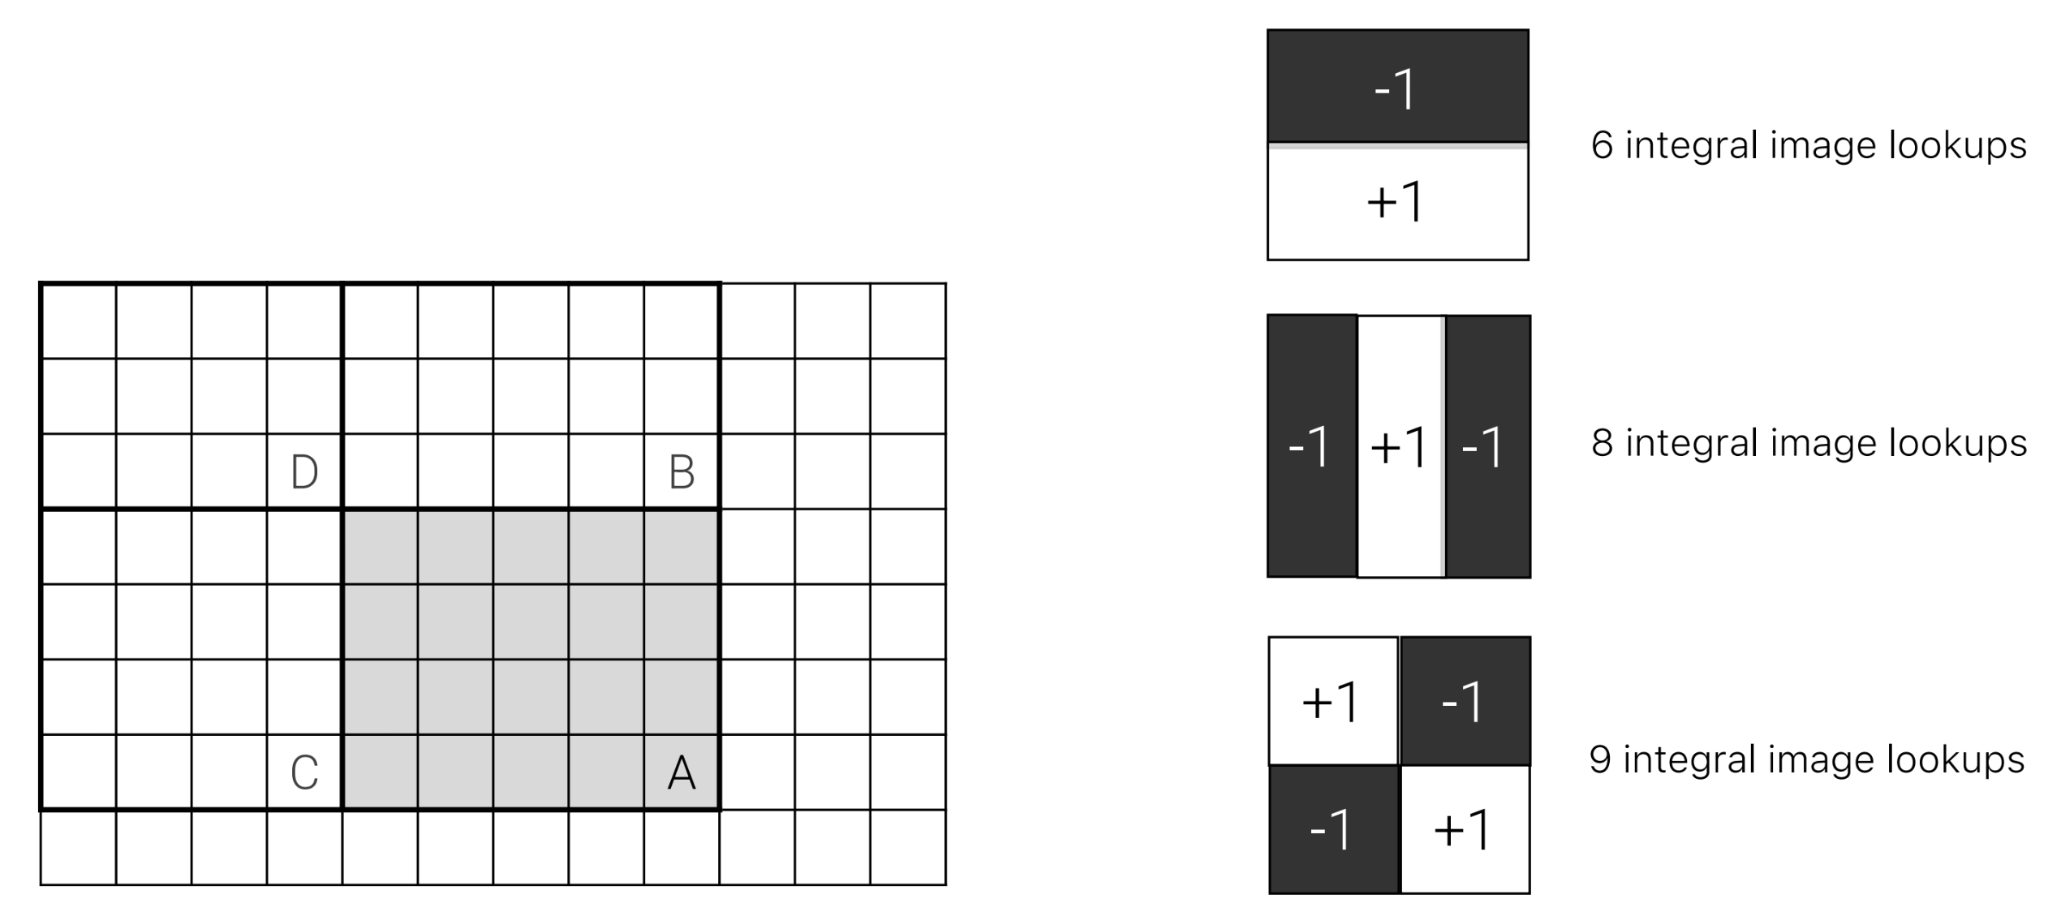
\includegraphics[width=0.6\linewidth]{./img/integral_filters.png}
  \caption{Rectangular filters can be computed in constant time with integral images}
\end{figure}

\paragraph{Multi-scale sliding window detector}
At test time, the strong classifier is applied to all spatial locations in the image.
Multi-scale detection is necessary, since faces are not necessarily $24\times 24$.
To achieve good performance, about 200 features are used to classify each patch.
Even if each feature can be computed very fast (thanks to integral images) there are still too many windows in an image to achieve real-time performance.

Faces are far less frequent in an image than background regions.
Most of the time is wasted computing a lot of features for background patches.
The key idea is then to reject most of the easy background patches with a simpler classifier which can be ran very fast.

\paragraph{Box overlap}

\begin{figure}[htbp]
  \centering
  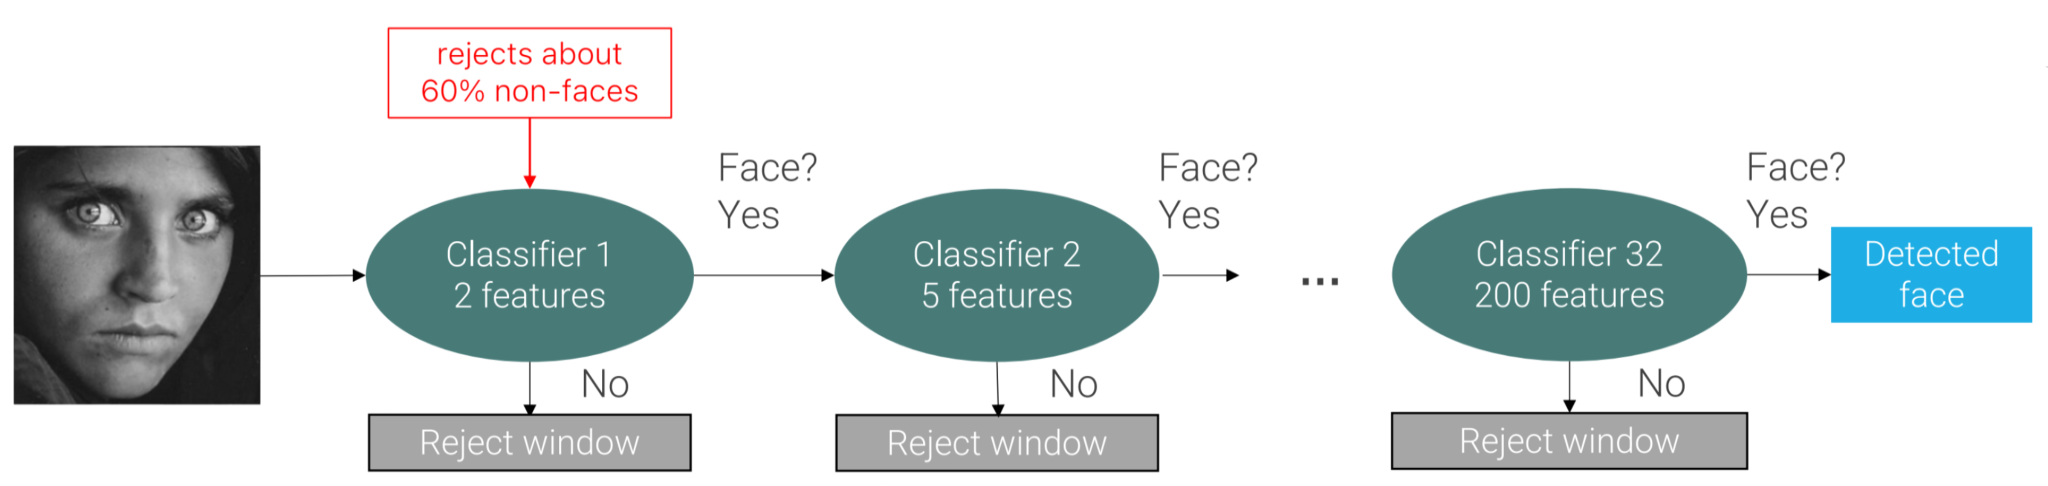
\includegraphics[width=0.6\linewidth]{./img/cascade_classifier.png}
  \caption{We use more and more features for face detection classifier after classifier}
\end{figure}

There will be several overlapping detections.
To check if two boxes overlap we measure the Intersection over Union ($IoU$) score: $IoU(BB_i, BB_j) = \frac{|BB_i \cap BB_j|}{|BB_i| + |BB_j| - |BB_i \cap BB_j|}$. $0.75$ corresponds to a good overlap, $0.90$ to a perfect one.
To obtain a single detection out of a set of overlapping boxes we perform Non Maxima Suppression of boxes.
Non Maxima Suppression considers the highest scoring Bounding Box, eliminates all the boxes with overlap greater than a threshold, and repeats this until all the boxes have been tested.

A detection is considered a True Positive if its overlap with the ground truth $BB^{GT}$ is greater than $\rho_{IoU}$.

\subsubsection{Transfer Learning}
If we can assume that only one object is present in the image, object detection simplifies to object localization.
Transfer learning is a technique where a model trained on one task is reused (or "transferred") for a different but related task.
Instead of training a model from scratch, you start with a pre-trained model and fine-tune it for your specific problem.
To solve object detection we can reuse any architecture used in image classification, by adding a regression head for predicting the bounding box.

We can apply a classification CNN as a sliding window detector.
We have to add a background class to discard background patches.
The problem is that there are too many boxes to try, since we have to try lots of positions with different scales and aspect ratios.
The solution is to use region proposals.

\subsubsection{Region proposals}
Region proposal algorithms inspect the image and attempt to find regions of an image that likely contain an object.
The algorithm as a first step oversegments the image into highly uniform regions, and then, based on similarity scores of color, texture and size it iteratively aggregates them.

\begin{figure}[htbp]
  \centering
  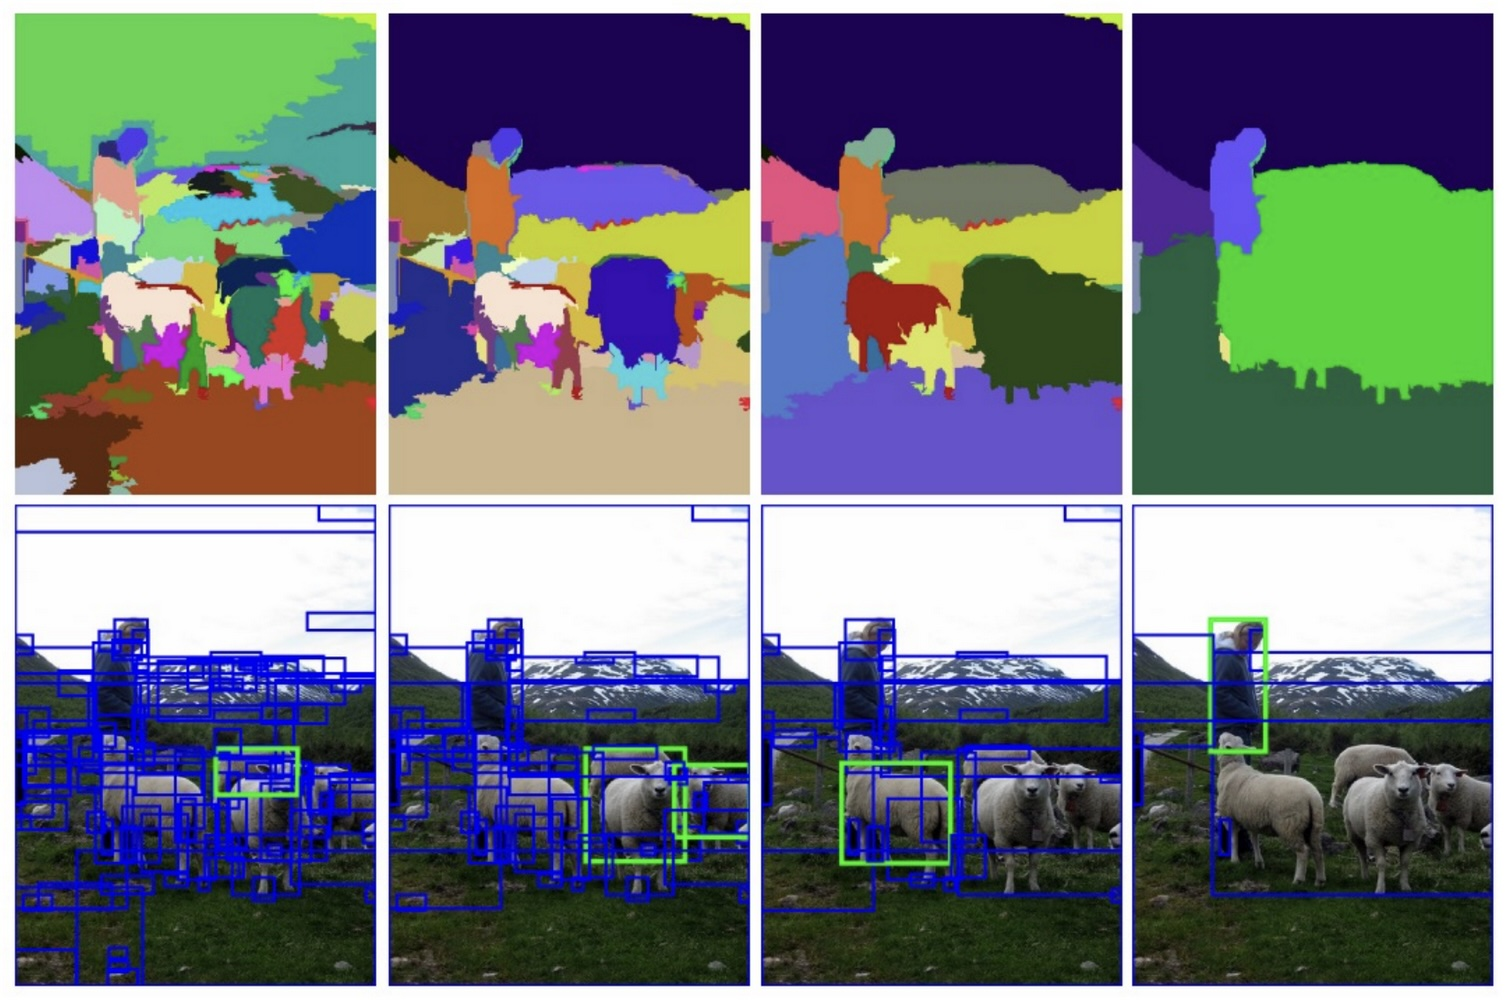
\includegraphics[width=0.6\linewidth]{./img/region_proposal.jpg}
  \caption{The 2 most similar regions are grouped together and then new similarities are calculated between the resulting region and its neighbours}
\end{figure}

\subsubsection{R-CNN: Region-based CNN}

Region-based CNN is the first object detector network.
As we can see in \ref{fig:rcnn} we run selective search to get about 2000 proposals, then we anisotropically (not uniformly across all directions) warp these proposals and add some pixels of context into a fixed size, to be able to input them in AlexNet, and for each proposal we get a class and a bounding box correction.

\begin{figure}[htbp]
  \centering
  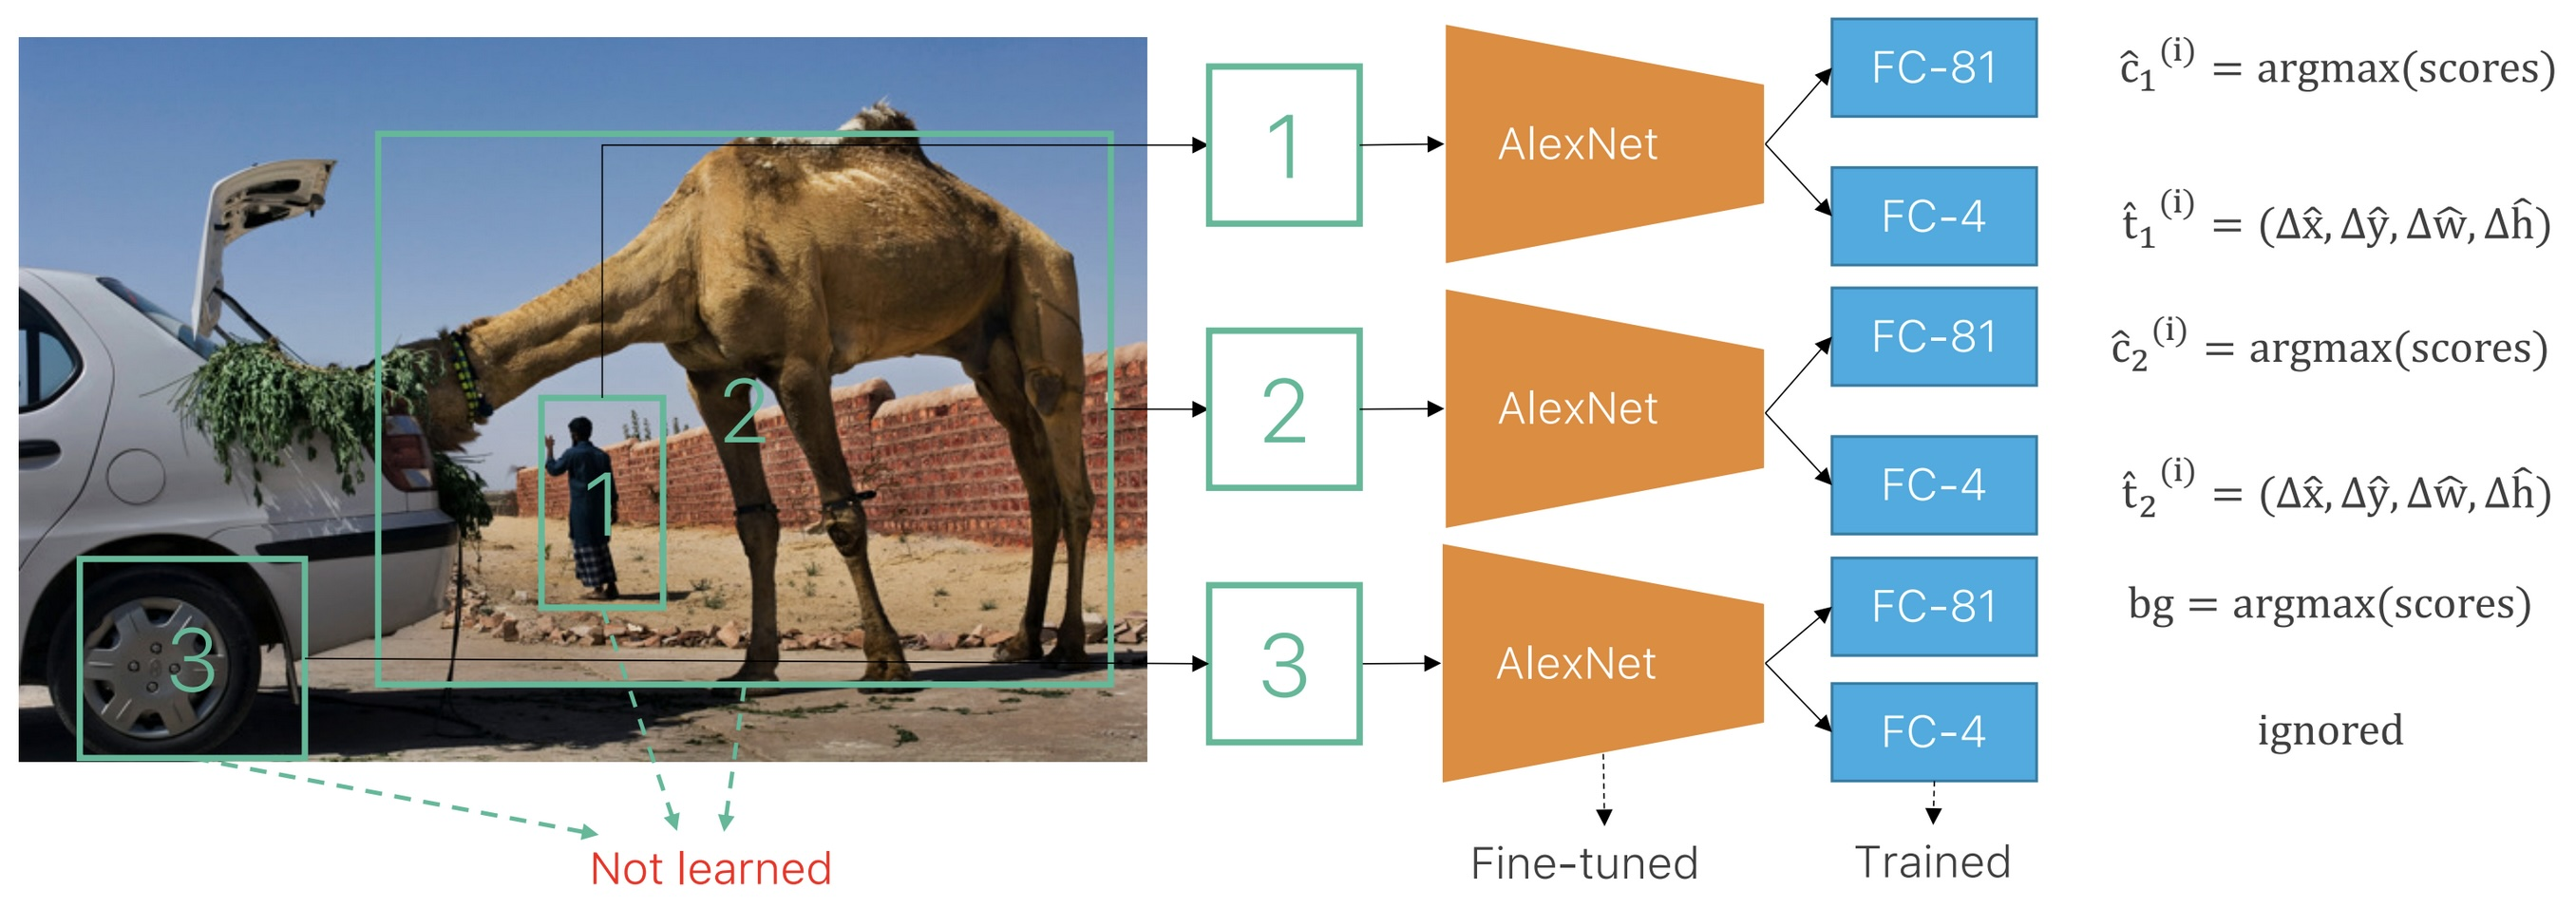
\includegraphics[width=0.6\linewidth]{./img/rcnn.jpg}
  \caption{R-CNN network architecture}
  \label{fig:rcnn}
\end{figure}

The problem is that since we have 2 different algorithms (one for the region proposal and one for AlexNet) we can't backpropagate through both of them.

\subsubsection{Fast R-CNN}

In the Fast R-CNN architecture showed in \ref{fig:fastrcnn} we can see that the model has been modified to run the first few layers of AlexNet on the original image, apply RoI pooling to crop and warp convolutional features according to proposal, and then run a small per-region network on each region to get the output class and bounding box correction.
This results in a faster networks since we don't have to apply 2000 CNN forward passes per image, but we apply most of the CNN before warping.

\begin{figure}[htbp]
  \centering
  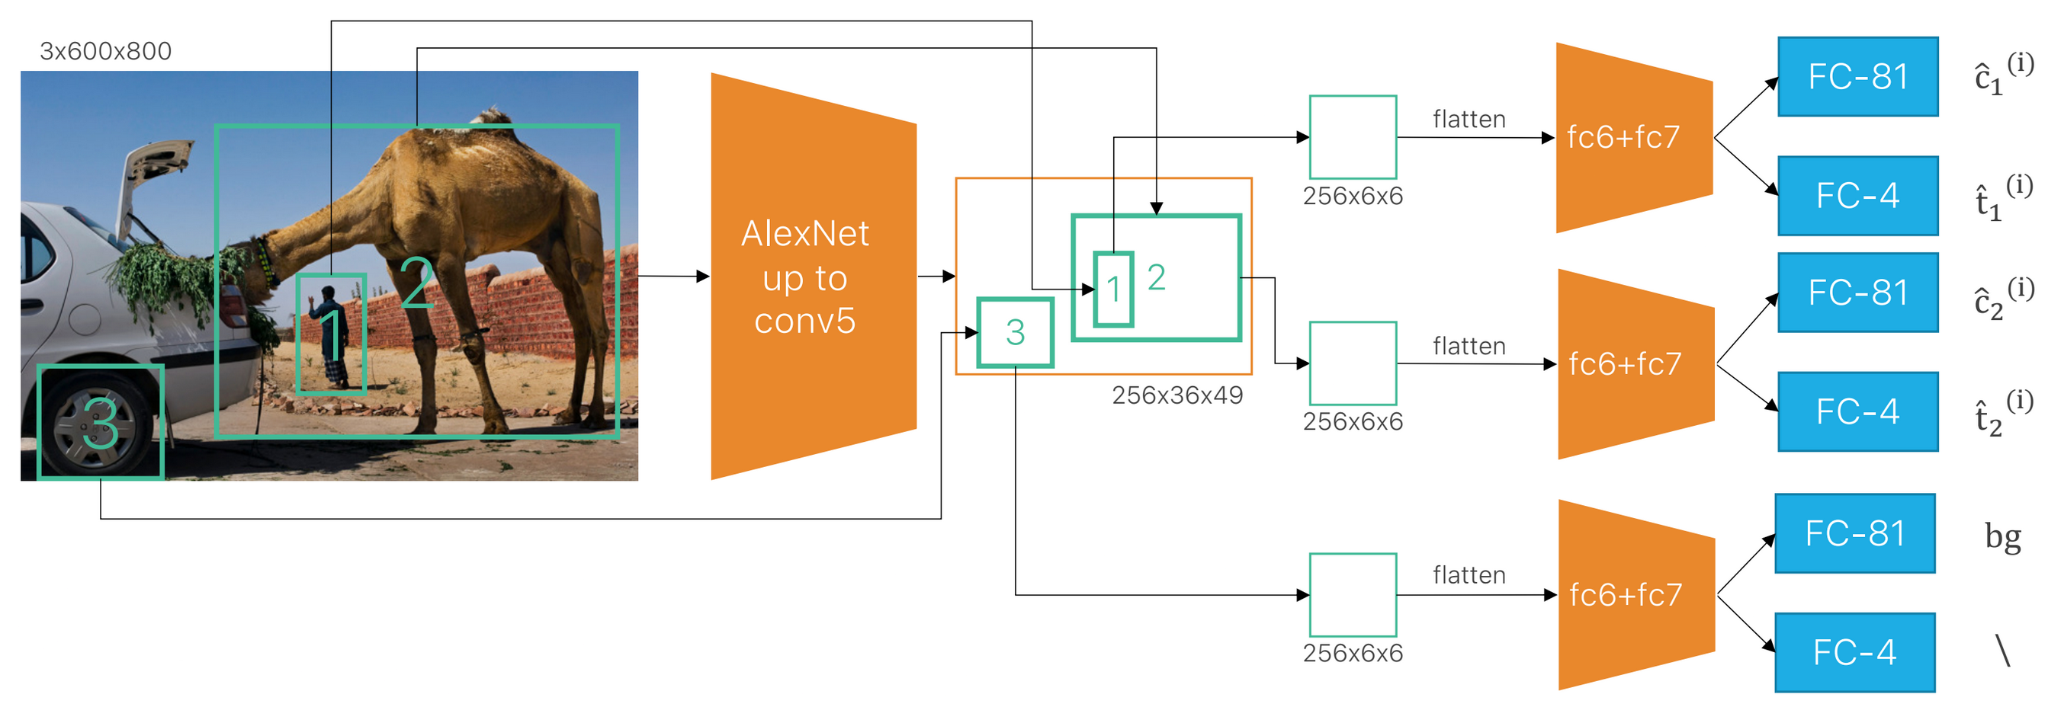
\includegraphics[width=0.6\linewidth]{./img/fastrcnn.png}
  \caption{Fast R-CNN network architecture}
  \label{fig:fastrcnn}
\end{figure}

Fast R-CNN uses the same bounding box correction of R-CNN, but with a smooth L1 loss (equal to L2 near the origin, but smoother elsewhere).

\paragraph{RoI pooling}
The RoIPool layer converts activations inside Region of Interest, corresponding to rescaled Selective Search regions, into activations with fixed spatial dimensions, which are the ones required by the remaining layers of the network.
To do RoI pooling, given a region:
\begin{enumerate}
  \item Snap the region to the grid.
  \item Apply max pooling kernels with approximate size $[H_r/H_o]\times [W_r/W_o]$ and approximate stride $s = [H_r/H_o]\times[W_r/W_o]$.
\end{enumerate}

\begin{figure}[htbp]
  \centering
  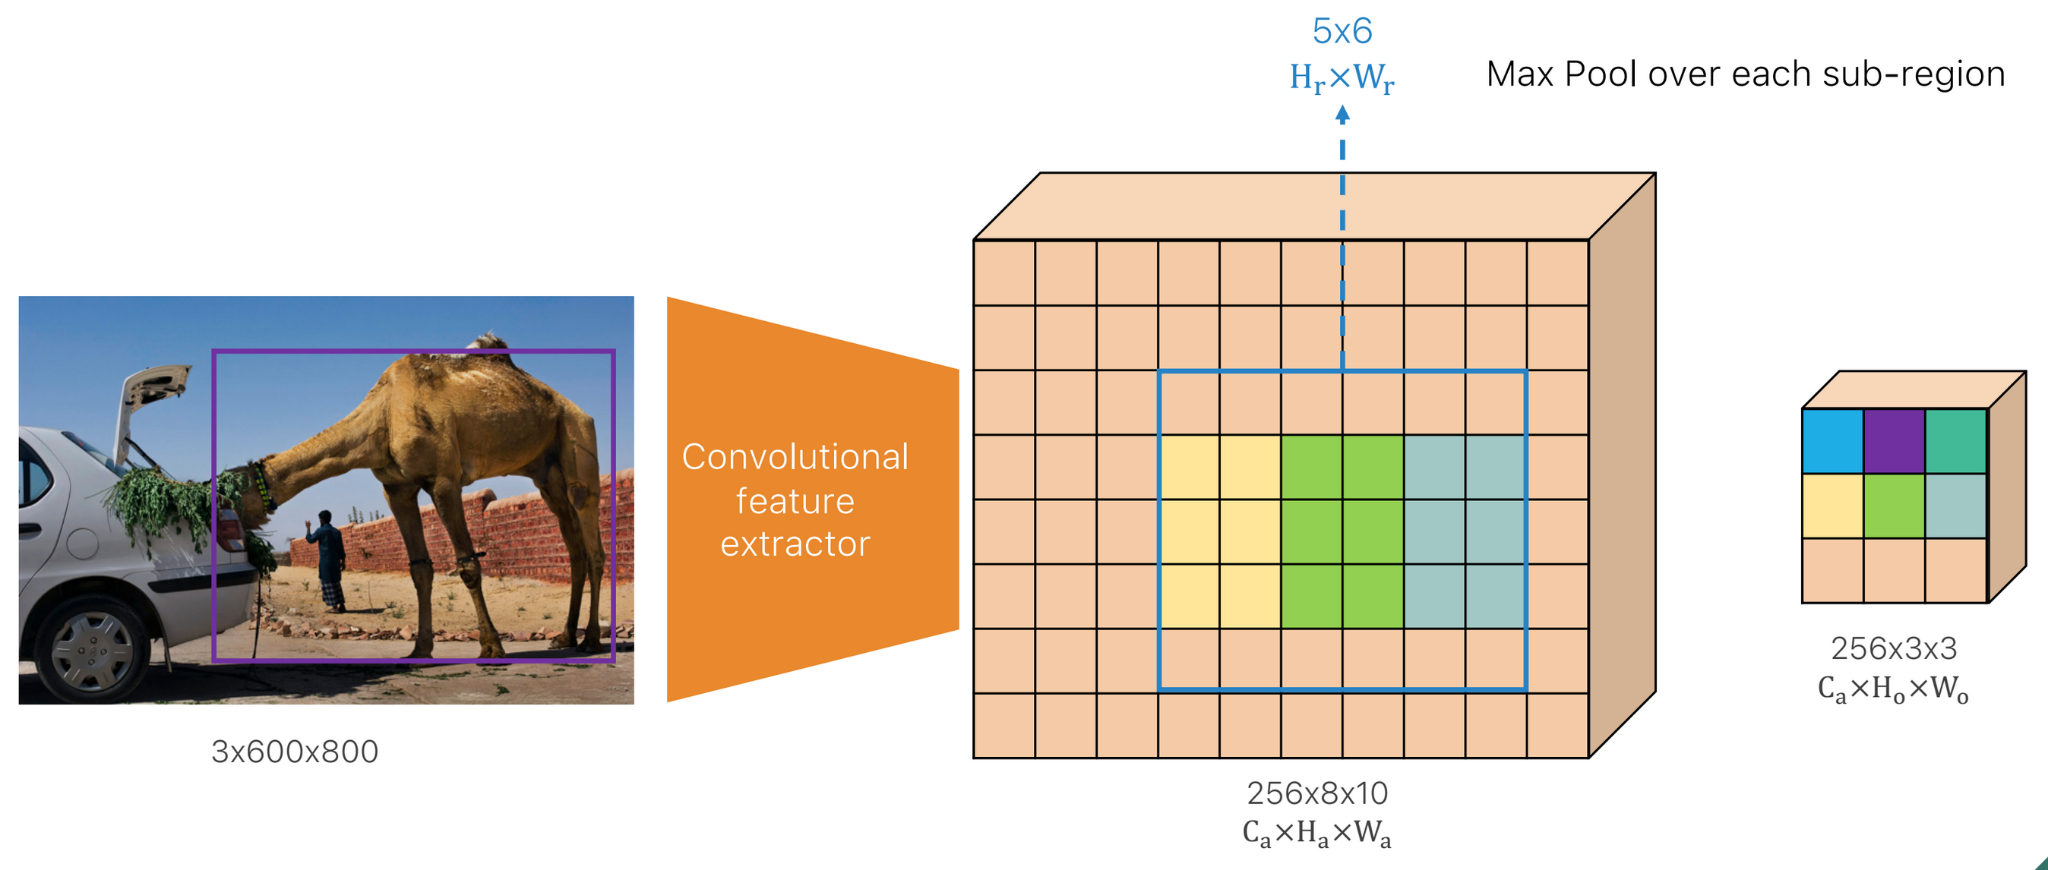
\includegraphics[width=0.6\linewidth]{./img/roipool.png}
  \caption{RoI pooling.}
\end{figure}

\subsubsection{Faster R-CNN}

In Fast R-CNN proposals are not learned, so the selective search is slow.
In Faster R-CNN they introduced a RPN (Region Proposal Network), which learns to predict the proposal box and the objectness score.

\begin{figure}[htbp]
  \centering
  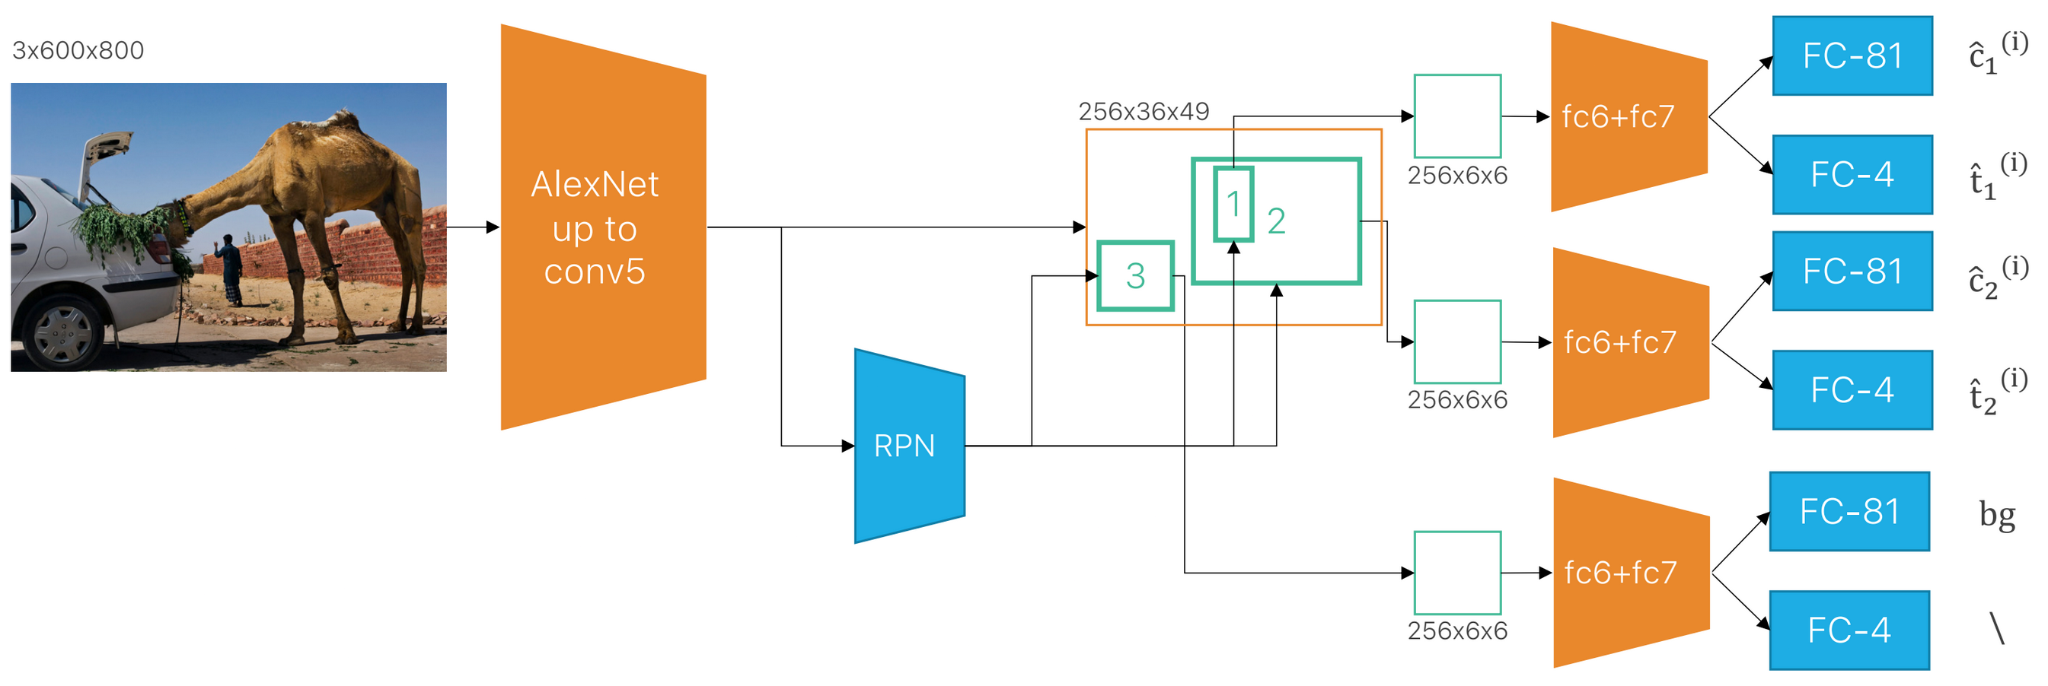
\includegraphics[width=0.6\linewidth]{./img/fasterrcnn.png}
  \caption{Faster R-CNN network architecture.}
\end{figure}

\paragraph{Region Proposal Network}

Region Proposal Networks are applied to a small $3\times 3$ window, which is approximately an object sized window in the original image and doesn't correspond to what we see in \ref{fig:rpn}, predicts the objectness and proposal bounding box.

\begin{figure}[htbp]
  \centering
  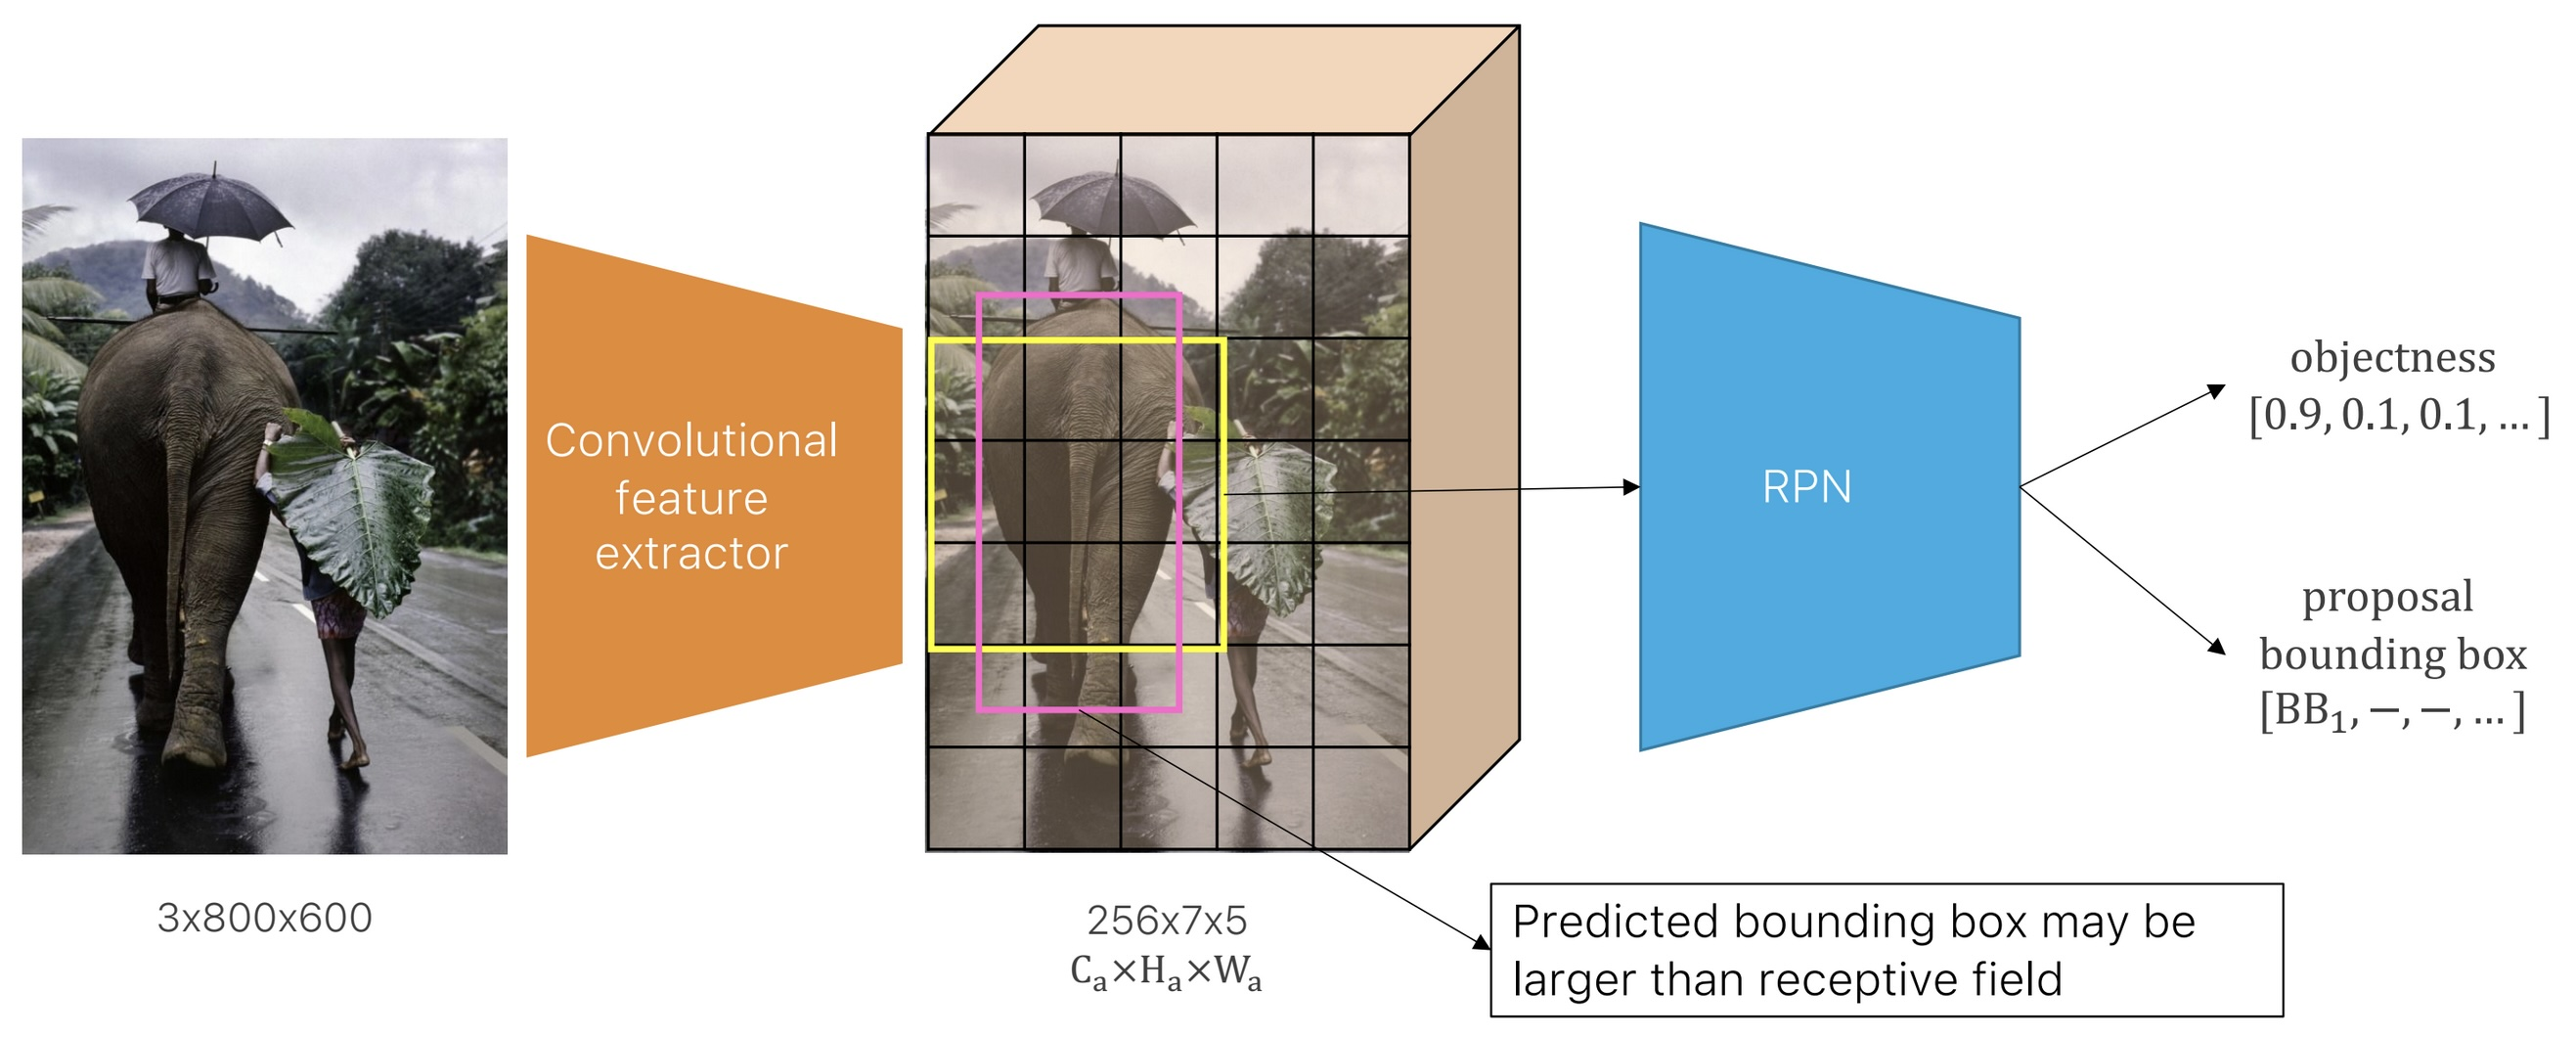
\includegraphics[width=0.6\linewidth]{./img/rpn.jpg}
  \caption{Region Proposal Network architecture.}
  \label{fig:rpn}
\end{figure}

When the objectness score is low, the localization head produces its output, but it's meaningless and it will be ignored.

\paragraph{Region Proposal Network with anchor}
We can simplify the creation of proposals.
An easier task may be to correct an input proposal, as done in R-CNN.

\begin{figure}[htbp]
  \centering
  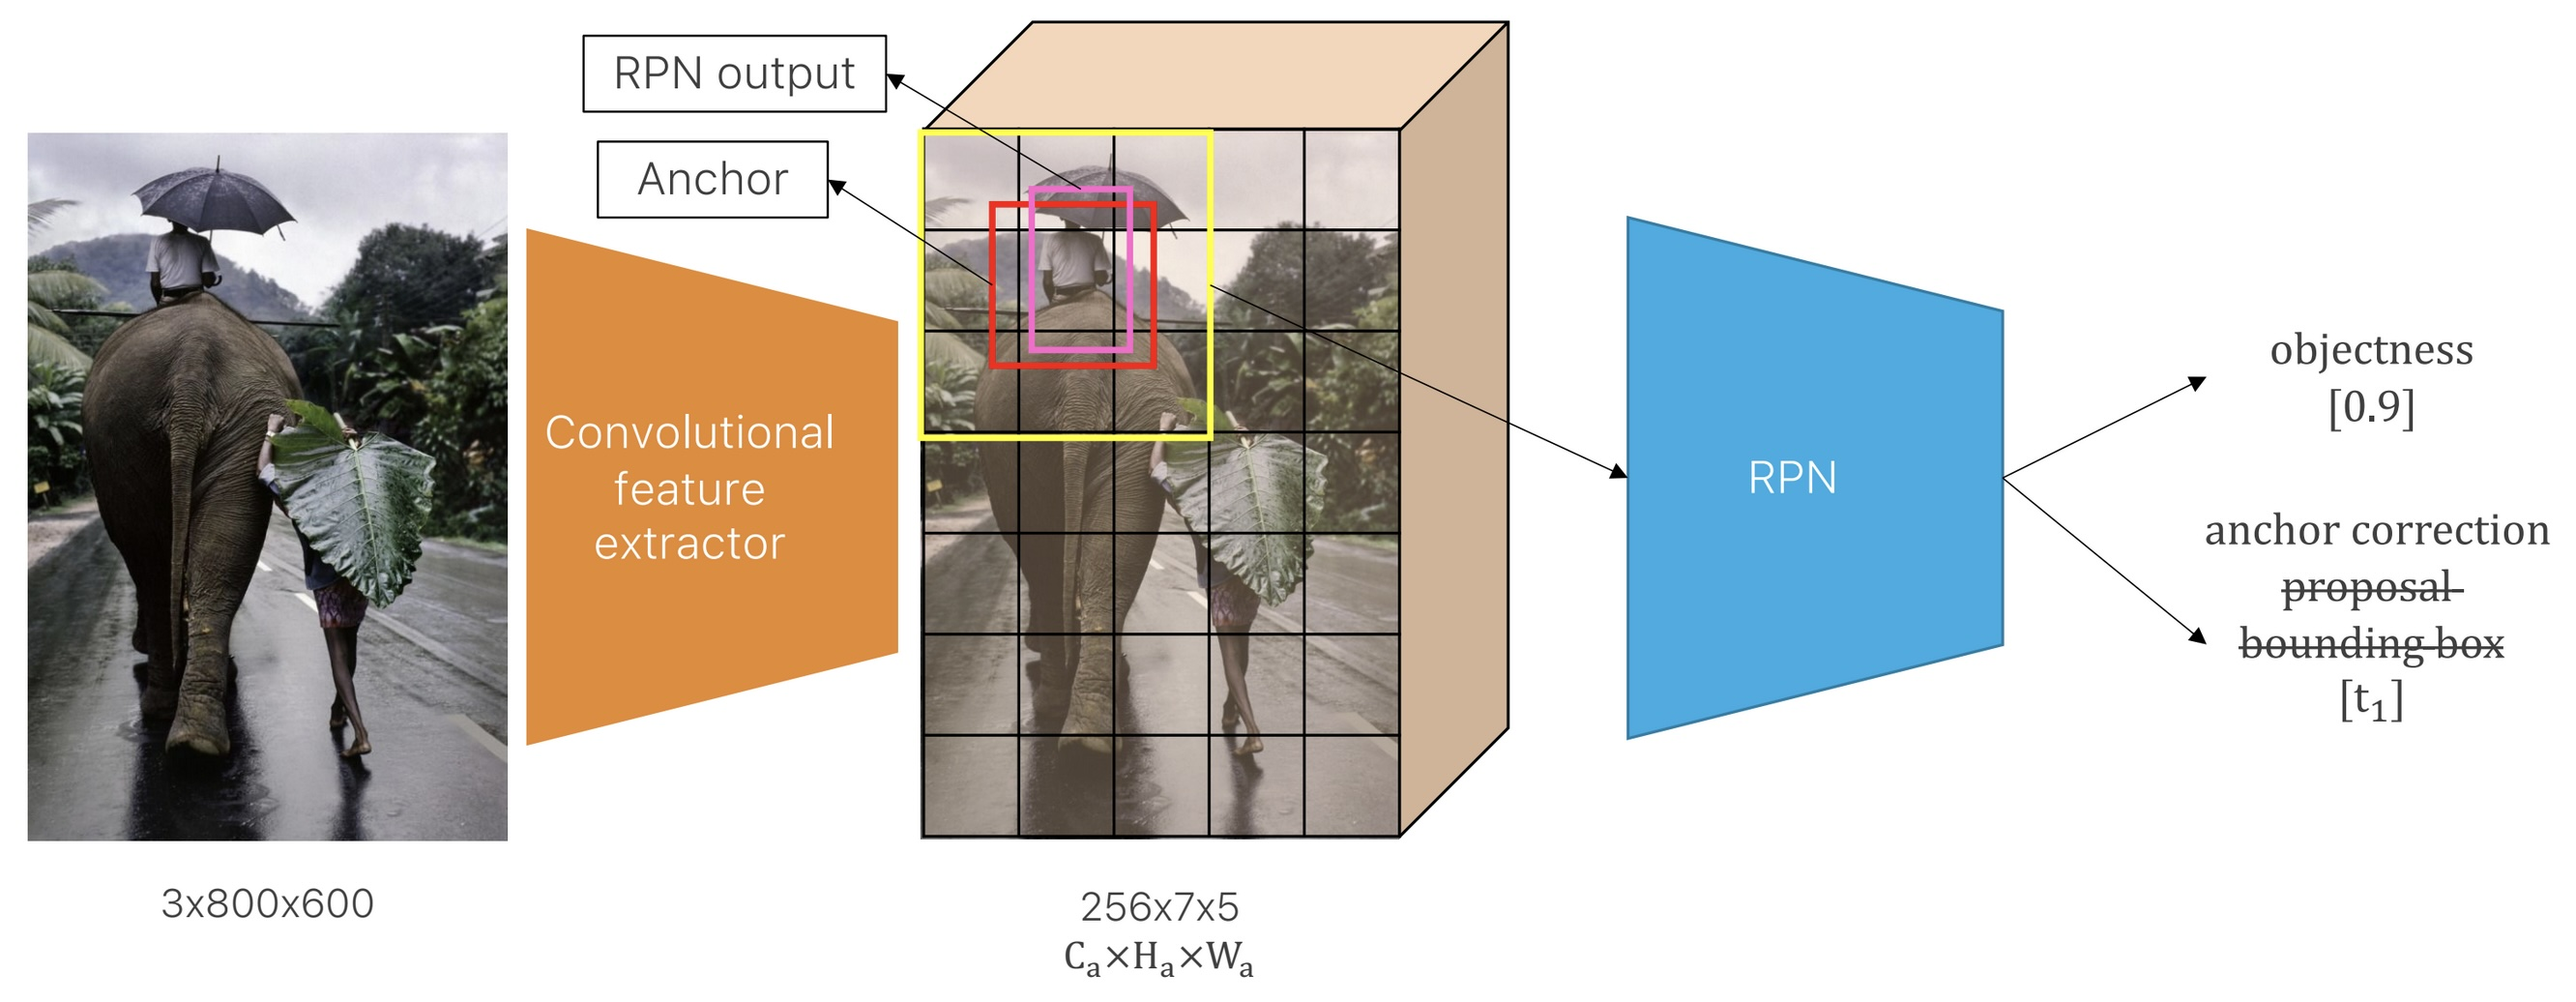
\includegraphics[width=0.6\linewidth]{./img/rpn_anchor.jpg}
  \caption{Our proposal here is a fixed scale and aspect-ratio box, known as anchor.}
\end{figure}

Objects have different scales and asepct ratios, so we use several anchors with different scale and aspect ratios.
The RPN predicts $k$ objectness scores and $k$ corrections.

When training RPNs, given an image and a ground truth bounding box if the anchor has a low IoU with all ground-truth boxes in an image, it's considered as background.

In standard Faster-RCNN, the RPN processes only the last activation of the feature extractor, which is a semantically rich signal since it includes higher level features than previous activations, but very coarse in spatial resolution.
Even if small scale anchors are provided, it may miss objects smaller than the grid size.

% slide 62/71
